\chapter{矩阵群与群作用}

本章进入与模形式最直接相关的一组代数对象：矩阵群、同余子群，以及它们在上半平面上的作用。对于模形式理论而言，$\SL_2(\Z)$ 及其各种子群并不是偶然出现的；它们一方面来自整数矩阵的代数结构，另一方面通过分式线性变换作用在 $\HH$ 上，从而把代数、几何与复分析联系起来。我们将从一般线性群与特殊线性群出发，证明 $\SL_2(\Z)$ 由两个基本矩阵生成，再引入合同子群、轨道与稳定子、Burnside 引理，以及标准基本域的构造。最后一节给出模曲线的几何直观图景，为后续模形式章节作准备。

\section{一般线性群 $\GL_n$ 与特殊线性群 $\SL_n$}

在线性代数中，$n\times n$ 可逆矩阵构成最基本的一类矩阵群。它们不仅本身重要，而且常常作为其他群的线性表示空间。

\begin{definition}
设 $F$ 是一个域，$n\ge 1$。定义
\[
\GL_n(F)=\{A\in M_n(F):\det A\ne 0\},
\]
称为 $F$ 上的\emph{一般线性群}。进一步定义
\[
\SL_n(F)=\{A\in \GL_n(F):\det A=1\},
\]
称为 $F$ 上的\emph{特殊线性群}。
\end{definition}

这里 $M_n(F)$ 表示所有 $n\times n$ 的 $F$-矩阵所成的集合。$\GL_n(F)$ 中的群运算就是矩阵乘法。

\begin{proposition}
对任意域 $F$ 与任意 $n\ge 1$，$\GL_n(F)$ 在矩阵乘法下构成一个群。
\end{proposition}

\begin{proof}
我们逐条验证群公理。

\begin{enumerate}
  \item \textbf{封闭性：}若 $A,B\in \GL_n(F)$，则 $\det A\ne 0$ 且 $\det B\ne 0$。由行列式的乘法公式，
  \[
  \det(AB)=\det(A)\det(B)\ne 0,
  \]
  因而 $AB\in \GL_n(F)$。

  \item \textbf{结合律：}矩阵乘法本身满足结合律，因此对 $\GL_n(F)$ 中的元素当然也成立。

  \item \textbf{单位元：}$n\times n$ 单位矩阵 $I_n$ 满足 $\det(I_n)=1\ne 0$，故 $I_n\in \GL_n(F)$，并且 $I_nA=AI_n=A$。

  \item \textbf{逆元：}若 $A\in \GL_n(F)$，则 $\det A\ne 0$。由伴随矩阵公式
  \[
  A^{-1}=\frac{1}{\det A}\operatorname{adj}(A),
  \]
  可知 $A$ 在 $M_n(F)$ 中可逆，因此 $A^{-1}\in \GL_n(F)$。事实上，
  \[
  \det(A^{-1})=(\det A)^{-1}\ne 0.
  \]
\end{enumerate}
故 $\GL_n(F)$ 是群。
\end{proof}

\begin{proposition}
行列式映射
\[
\det:\GL_n(F)\longrightarrow F^\times
\]
是群同态，其中 $F^\times=F\setminus\{0\}$ 在乘法下成群。
\end{proposition}

\begin{proof}
对任意 $A,B\in \GL_n(F)$，有
\[
\det(AB)=\det(A)\det(B),
\]
这正是群同态的定义。又因 $A\in \GL_n(F)$ 当且仅当 $\det A\in F^\times$，所以该映射确实以 $F^\times$ 为值域。
\end{proof}

\begin{theorem}
$\SL_n(F)$ 是 $\GL_n(F)$ 的正规子群，并且
\[
\GL_n(F)/\SL_n(F)\cong F^\times.
\]
\end{theorem}

\begin{proof}
由上一个命题，$\SL_n(F)=\ker(\det)$。任何群同态的核都是正规子群，因此 $\SL_n(F)\trianglelefteq \GL_n(F)$。又因为行列式映射是满射：对任意 $\lambda\in F^\times$，矩阵
\[
\operatorname{diag}(\lambda,1,\dots,1)\in \GL_n(F)
\]
满足 $\det=\lambda$。于是由群同态基本定理得
\[
\GL_n(F)/\ker(\det)\cong \operatorname{im}(\det)=F^\times,
\]
即
\[
\GL_n(F)/\SL_n(F)\cong F^\times.
\]
\end{proof}

\begin{remark}
这一结论告诉我们：$\GL_n(F)$ 与 $\SL_n(F)$ 的差别，恰好由“行列式这一一维信息”控制。换言之，若把行列式忽略掉，$\GL_n(F)$ 就被压缩为 $\SL_n(F)$。
\end{remark}

\begin{example}
在实数域上，
\[
\GL_n(\R)=\{A:\det A\ne 0\}
\]
分成两部分：$\det A>0$ 与 $\det A<0$。因此
\[
\GL_n(\R)/\SL_n(\R)\cong \R^\times,
\]
但从连通性的角度看，$\GL_n(\R)$ 的两个连通分支对应于行列式的符号。
\end{example}

\begin{example}
在复数域上，$\C^\times$ 是连通的，因此 $\GL_n(\C)$ 与 $\SL_n(\C)$ 的关系更像“一个连续的标量参数”的扩张。特别地，任何非零复数都可以作为某个可逆复矩阵的行列式。
\end{example}

\begin{example}
在有限域 $\F_p$ 上，$\GL_n(\F_p)$ 与 $\SL_n(\F_p)$ 都是有限群。例如当 $n=1$ 时，
\[
\GL_1(\F_p)=\F_p^\times,
\qquad
\SL_1(\F_p)=\{1\}.
\]
当 $n=2$ 时，$\GL_2(\F_p)$ 是所有可逆 $2\times 2$ 模 $p$ 矩阵所成的有限群，而 $\SL_2(\F_p)$ 是其中行列式等于 $1$ 的子群。
\end{example}

\begin{proposition}
设 $q$ 是素数幂。则
\[
|\GL_n(\F_q)|=(q^n-1)(q^n-q)\cdots(q^n-q^{n-1}).
\]
等价地，
\[
|\GL_n(\F_q)|=q^{n^2}\prod_{j=1}^n\left(1-q^{-j}\right).
\]
\end{proposition}

\begin{proof}
把一个 $n\times n$ 矩阵看成由 $n$ 个列向量组成。矩阵可逆当且仅当这 $n$ 个列向量在 $\F_q^n$ 中线性无关。

第一列可以是任意非零向量，共有 $q^n-1$ 种取法。取定前 $k$ 列线性无关后，它们张成一个 $k$ 维子空间，其中共有 $q^k$ 个向量。因此第 $k+1$ 列必须避开这个子空间，所以有 $q^n-q^k$ 种取法。依次相乘，得到
\[
|\GL_n(\F_q)|=(q^n-1)(q^n-q)\cdots(q^n-q^{n-1}).
\]

把第 $j$ 个因子写成 $q^n(1-q^{-j})$ 的形式，便得到第二个表达式。更精确地，
\[
(q^n-1)(q^n-q)\cdots(q^n-q^{n-1})
= q^{0+1+\cdots+(n-1)}\prod_{j=1}^n(q^j-1),
\]
再整理即可得到所述公式。
\end{proof}

\begin{corollary}
对有限域 $\F_q$，有
\[
|\SL_n(\F_q)|=\frac{|\GL_n(\F_q)|}{q-1}.
\]
特别地，
\[
|\SL_2(\F_q)|=q(q^2-1).
\]
\end{corollary}

\begin{proof}
行列式映射
\[
\det:\GL_n(\F_q)\to \F_q^\times
\]
是满同态，而 $|\F_q^\times|=q-1$。所以
\[
|\GL_n(\F_q)|=|\SL_n(\F_q)|\cdot(q-1).
\]
当 $n=2$ 时，
\[
|\GL_2(\F_q)|=(q^2-1)(q^2-q)=q(q-1)(q^2-1),
\]
故
\[
|\SL_2(\F_q)|=q(q^2-1).
\]
\end{proof}

\begin{example}
取 $q=2$，则
\[
|\GL_2(\F_2)|=(2^2-1)(2^2-2)=3\cdot 2=6,
\qquad
|\SL_2(\F_2)|=6.
\]
这是因为 $\F_2^\times=\{1\}$，所以在 $\F_2$ 上行列式自动等于 $1$。

取 $q=3$，则
\[
|\GL_2(\F_3)|=(9-1)(9-3)=8\cdot 6=48,
\qquad
|\SL_2(\F_3)|=24.
\]
\end{example}

\section{$\SL_2(\Z)$ 的生成元}

从本节开始，我们把注意力集中到
\[
\SL_2(\Z)=\left\{\mat{a&b\\ c&d}:a,b,c,d\in\Z,\ ad-bc=1\right\}.
\]
这是模形式理论中最核心的离散群。它有两个极其重要的元素：
\[
S=\mat{0&-1\\ 1&0},
\qquad
T=\mat{1&1\\ 0&1}.
\]

\begin{proposition}
矩阵 $S,T$ 都属于 $\SL_2(\Z)$，并满足
\[
S^2=-I,
\qquad
S^4=I,
\qquad
(ST)^3=-I.
\]
因此在 $\PSL_2(\Z)=\SL_2(\Z)/\{\pm I\}$ 中有关系
\[
\bar S^2=\Id,
\qquad
(\bar S\bar T)^3=\Id.
\]
\end{proposition}

\begin{proof}
先算行列式：
\[
\det S=(0)(0)-(-1)(1)=1,
\qquad
\det T=(1)(1)-(1)(0)=1,
\]
故 $S,T\in \SL_2(\Z)$。

直接计算得
\[
S^2=
\mat{0&-1\\ 1&0}
\mat{0&-1\\ 1&0}
=
\mat{-1&0\\ 0&-1}
=-I,
\]
于是 $S^4=(-I)^2=I$。

再算
\[
ST=
\mat{0&-1\\ 1&0}
\mat{1&1\\ 0&1}
=
\mat{0&-1\\ 1&1}.
\]
进而
\[
(ST)^2=
\mat{0&-1\\ 1&1}
\mat{0&-1\\ 1&1}
=
\mat{-1&-1\\ 1&0},
\]
以及
\[
(ST)^3=
\mat{-1&-1\\ 1&0}
\mat{0&-1\\ 1&1}
=
\mat{-1&0\\ 0&-1}
=-I.
\]
在商群 $\PSL_2(\Z)$ 中，$-I$ 与 $I$ 同类，因此得到所述关系。
\end{proof}

\begin{example}
矩阵 $T^m$ 的形式非常简单：
\[
T^m=\mat{1&m\\ 0&1}\qquad (m\in\Z).
\]
又因为 $S^{-1}=-S$，所以
\[
STS^{-1}=\mat{1&0\\ -1&1},
\qquad
ST^{-m}S^{-1}=\mat{1&0\\ m&1}.
\]
这说明 $S$ 与 $T$ 能产生上三角与下三角两类基本幺模矩阵。
\end{example}

\begin{theorem}
$\SL_2(\Z)$ 由 $S$ 与 $T$ 生成。
\end{theorem}

\begin{proof}
设
\[
A=\mat{a&b\\ c&d}\in \SL_2(\Z).
\]
我们对 $|c|$ 作归纳，证明 $A$ 可写成 $S,T$ 的字。

\medskip
\noindent\textbf{第一步：基例 $c=0$.}
此时由 $ad-bc=1$ 得 $ad=1$，故 $a=d=\pm 1$。

若 $a=d=1$，则
\[
A=\mat{1&b\\ 0&1}=T^b.
\]
若 $a=d=-1$，则
\[
A=\mat{-1&b\\ 0&-1}=-\mat{1&-b\\ 0&1}=S^2T^{-b}.
\]
因此当 $c=0$ 时，命题成立。

\medskip
\noindent\textbf{第二步：归纳步骤。}
设命题对所有满足 $|c'|<|c|$ 的矩阵都成立，其中 $c\ne 0$。我们证明它也对 $A$ 成立。

根据整数除法，可以取某个 $q\in\Z$，使得
\[
|a-qc|\le \frac{|c|}{2}.
\]
考虑左乘 $T^{-q}$：
\[
T^{-q}A=
\mat{1&-q\\ 0&1}
\mat{a&b\\ c&d}
=
\mat{a-qc&b-qd\\ c&d}.
\]
再左乘 $S$，得
\[
A_1\coloneqq ST^{-q}A
=
\mat{0&-1\\ 1&0}
\mat{a-qc&b-qd\\ c&d}
=
\mat{-c&-d\\ a-qc&b-qd}.
\]
这是 $\SL_2(\Z)$ 中的矩阵，其左下角元素是 $a-qc$。由于它是整数且满足
\[
|a-qc|\le \frac{|c|}{2}<|c|,
\]
可知 $A_1$ 的左下角绝对值严格小于 $|c|$。由归纳假设，$A_1$ 可由 $S,T$ 生成。

于是
\[
A=(ST^{-q})^{-1}A_1=T^qS^{-1}A_1.
\]
而 $S^{-1}=-S=S^3$ 属于由 $S$ 生成的子群，因此 $A$ 也可由 $S,T$ 生成。

由数学归纳法，$\SL_2(\Z)=\langle S,T\rangle$。
\end{proof}

\begin{remark}
上述证明本质上是欧几里得算法在矩阵上的表现。它不断把矩阵左下角的整数 $c$ 变小，直到降为 $0$，这与用初等整数变换求最大公因数完全同型。
\end{remark}

\begin{example}
设
\[
A=\mat{2&1\\ 1&1}.
\]
因为
\[
ST^{-1}=
\mat{0&-1\\ 1&-1},
\qquad
(ST^{-1})A=
\mat{-1&-1\\ 1&0},
\]
再乘以 $T$ 就能进一步化简。实际上容易验证
\[
A=TS^{-1}T.
\]
读者可以把本节定理中的归纳步骤具体执行一遍，体会“把任意矩阵写成 $S,T$ 的字”的算法性。
\end{example}

\section{合同子群 $\Gamma(N)$, $\Gamma_0(N)$, $\Gamma_1(N)$}

模形式通常不是对整个 $\SL_2(\Z)$ 而言，而是对它的某个有限指标子群而言。最重要的一类便是\emph{合同子群}。

\begin{definition}
设 $N\ge 1$。定义 $\SL_2(\Z)$ 的三个子集：
\[
\Gamma(N)=\left\{\mat{a&b\\ c&d}\in \SL_2(\Z):
\mat{a&b\\ c&d}\equiv \mat{1&0\\ 0&1}\pmod N\right\},
\]
\[
\GammaO(N)=\left\{\mat{a&b\\ c&d}\in \SL_2(\Z):c\equiv 0\pmod N\right\},
\]
\[
\GammaI(N)=\left\{\mat{a&b\\ c&d}\in \SL_2(\Z):a\equiv d\equiv 1\pmod N,\ c\equiv 0\pmod N\right\}.
\]
其中 $\Gamma(N)$ 称为\emph{主合同子群}，$\GammaO(N)$ 称为\emph{Hecke 合同子群}，$\GammaI(N)$ 称为\emph{带一个截面的合同子群}。
\end{definition}

\begin{proposition}
对每个 $N\ge 1$，$\Gamma(N)$、$\GammaO(N)$、$\GammaI(N)$ 都是 $\SL_2(\Z)$ 的子群，并且
\[
\Gamma(N)\trianglelefteq \SL_2(\Z),
\qquad
\Gamma(N)\subseteq \GammaI(N)\subseteq \GammaO(N).
\]
\end{proposition}

\begin{proof}
先证它们是子群。设
\[
A=\mat{a&b\\ c&d},\qquad B=\mat{a'&b'\\ c'&d'}.
\]
若 $A,B\in \GammaO(N)$，则
\[
AB=\mat{aa'+bc'&ab'+bd'\\ ca'+dc'&cb'+dd'}.
\]
其左下角是 $ca'+dc'$，显然仍被 $N$ 整除，所以 $AB\in \GammaO(N)$。又
\[
A^{-1}=\mat{d&-b\\ -c&a},
\]
其左下角为 $-c$，仍被 $N$ 整除，因此 $\GammaO(N)$ 是子群。

同理，若 $A,B\in \GammaI(N)$，则它们的左下角仍被 $N$ 整除，且对角元模 $N$ 仍等于 $1$，逆矩阵的对角元也分别是 $d,a\equiv 1\pmod N$，故 $\GammaI(N)$ 是子群。

对 $\Gamma(N)$，它是下面模 $N$ 约化映射的核，因此自动是正规子群。集合包含关系则从定义直接可见。
\end{proof}

\begin{definition}
设 $N\ge 1$。把矩阵各个元素按模 $N$ 约化，得到映射
\[
\rho_N:\SL_2(\Z)\longrightarrow \SL_2(\Z/N\Z),
\qquad
\mat{a&b\\ c&d}\longmapsto \mat{\bar a&\bar b\\ \bar c&\bar d}.
\]
称为\emph{模 $N$ 约化映射}。
\end{definition}

\begin{proposition}
$\rho_N$ 是群同态，且
\[
\ker(\rho_N)=\Gamma(N).
\]
\end{proposition}

\begin{proof}
矩阵乘法与模 $N$ 约化可交换，因此 $\rho_N(AB)=\rho_N(A)\rho_N(B)$，故 $\rho_N$ 是群同态。

另一方面，$A\in \ker(\rho_N)$ 当且仅当 $A$ 的每个元素模 $N$ 与单位矩阵对应元素相同，即
\[
A\equiv I \pmod N.
\]
这正是 $A\in \Gamma(N)$ 的定义。所以 $\ker(\rho_N)=\Gamma(N)$。
\end{proof}

下面的满射性非常重要，它说明 $\SL_2(\Z)$ 在模 $N$ 的意义下已经“覆盖”了全部的 $\SL_2(\Z/N\Z)$。

\begin{theorem}
对任意 $N\ge 1$，约化映射
\[
\rho_N:\SL_2(\Z)\to \SL_2(\Z/N\Z)
\]
是满射。
\end{theorem}

\begin{proof}
取任意矩阵
\[
\bar A=\mat{\bar a&\bar b\\ \bar c&\bar d}\in \SL_2(\Z/N\Z),
\]
即满足
\[
\bar a\bar d-\bar b\bar c=1
\]
于环 $\Z/N\Z$ 中成立。

我们首先证明：可以选取整数 $c,d$，使得
\[
c\equiv \bar c\pmod N,
\qquad d\equiv \bar d\pmod N,
\qquad \gcd(c,d)=1.
\]
先任意取整数提升 $c_0,d_0$。由 $\bar a\bar d-\bar b\bar c=1$ 可知理想 $(\bar c,\bar d)$ 生成整个环 $\Z/N\Z$；等价地，对每个素数 $p\mid N$，$\bar c,\bar d$ 不可能同时被 $p$ 整除。因此当 $p\mid N$ 且 $p\mid c_0$ 时，必有 $p\nmid d_0$。

现在只需通过替换 $d_0$ 为 $d_0+Nt$ 来消去 $\gcd(c_0,d_0)$ 中那些不整除 $N$ 的素因子。设 $p_1,\dots,p_r$ 是所有整除 $c_0$ 但不整除 $N$ 的不同素数。对每个 $p_i$，因为 $N$ 在模 $p_i$ 下可逆，所以同余式
\[
d_0+Nt\equiv 0\pmod{p_i}
\]
至多有一个解类。于是我们可以选取整数 $t$，使得对每个 $i$ 都有 $d_0+Nt\not\equiv 0\pmod{p_i}$。令
\[
d=d_0+Nt,
\qquad c=c_0.
\]
则 $c\equiv \bar c$, $d\equiv \bar d\pmod N$，并且任何整除 $c,d$ 的素数都不能整除 $N$，又被我们排除掉，所以 $\gcd(c,d)=1$。

既然 $\gcd(c,d)=1$，由 Bézout 等式存在整数 $a_0,b_0$，使得
\[
a_0d-b_0c=1.
\]
再任取整数提升 $\tilde a,\tilde b$，满足
\[
\tilde a\equiv \bar a\pmod N,
\qquad \tilde b\equiv \bar b\pmod N.
\]
由于 $\tilde a d-\tilde b c\equiv 1\pmod N$，可得
\[
d(\tilde a-a_0)-c(\tilde b-b_0)\equiv 0\pmod N.
\]
取整数 $u,v$ 使 $uc+vd=1$。设
\[
t=u(\tilde a-a_0)+v(\tilde b-b_0).
\]
则
\[
ct\equiv \tilde a-a_0 \pmod N,
\qquad
dt\equiv \tilde b-b_0 \pmod N.
\]
于是令
\[
a=a_0+ct,
\qquad b=b_0+dt.
\]
便有
\[
a\equiv \tilde a\equiv \bar a\pmod N,
\qquad b\equiv \tilde b\equiv \bar b\pmod N,
\]
并且
\[
ad-bc=(a_0+ct)d-(b_0+dt)c=a_0d-b_0c=1.
\]
故
\[
A=\mat{a&b\\ c&d}\in \SL_2(\Z)
\]
且 $\rho_N(A)=\bar A$。满射性得证。
\end{proof}

\begin{remark}
因此 $\Gamma(N)$ 的确是有限指标正规子群，而且
\[
\SL_2(\Z)/\Gamma(N)\cong \SL_2(\Z/N\Z).
\]
从模形式的观点看，$\Gamma(N)$ 对应“带完全 $N$ 级结构”的对象，而 $\GammaO(N),\GammaI(N)$ 则对应较弱的级结构。
\end{remark}

为了计算 $\GammaO(N)$ 的指标，我们引入射影直线。

\begin{definition}
记 $R=\Z/N\Z$。定义 $\mathbf{P}^1(R)$ 为所有\emph{原始对} $(x,y)\in R^2$ 的等价类集合，其中“原始”指 $x,y$ 生成整个环 $R$ 的单位理想；等价关系规定为
\[
(x,y)\sim (ux,uy)\qquad (u\in R^\times).
\]
我们把等价类记作 $[x:y]$。
\end{definition}

\begin{proposition}
群 $\SL_2(\Z/N\Z)$ 作用在 $\mathbf{P}^1(\Z/N\Z)$ 上，并且该作用是传递的。点 $[1:0]$ 的稳定子恰好是上三角子群
\[
B(N)=\left\{\mat{a&b\\ 0&d}\in \SL_2(\Z/N\Z)\right\}.
\]
\end{proposition}

\begin{proof}
矩阵对列向量的左乘保持原始性，因此诱导出对射影类的作用。

取任意原始类 $[x:y]$。因为 $(x,y)$ 原始，所以理想 $(x,y)=R$。按上面满射性证明中的同样方法，可构造矩阵
\[
\mat{x&*\\ y&*}\in \SL_2(R),
\]
于是该矩阵把 $[1:0]$ 送到 $[x:y]$，故作用传递。

再看稳定子。若
\[
A=\mat{a&b\\ c&d}
\]
固定 $[1:0]$，则
\[
A\binom{1}{0}=\binom{a}{c}
\]
必须与 $\binom{1}{0}$ 成比例，因此必有 $c=0$。反过来，若 $c=0$，则
\[
A\binom{1}{0}=\binom{a}{0}
\]
与 $\binom{1}{0}$ 确实代表同一点。于是稳定子正是 $B(N)$。
\end{proof}

\begin{lemma}
若 $N=p^r$ 是素数幂，则
\[
\bigl|\mathbf{P}^1(\Z/p^r\Z)\bigr|=p^r+p^{r-1}.
\]
\end{lemma}

\begin{proof}
设 $R=\Z/p^r\Z$。任取原始类 $[x:y]$。

若 $y$ 是单位，则把它缩放为 $1$，可唯一写成 $[u:1]$，其中 $u\in R$，共 $p^r$ 个。

若 $y$ 不是单位，则 $p\mid y$。由于 $(x,y)$ 原始，必有 $x$ 是单位，于是可缩放为 $[1:v]$。此时 $v$ 必须被 $p$ 整除；反之每个这样的 $v$ 都给出一个原始类。被 $p$ 整除的元素恰有 $p^{r-1}$ 个。

这两类互不相交，因为第一类中第二坐标是单位，第二类中第二坐标不是单位。因此
\[
\bigl|\mathbf{P}^1(R)\bigr|=p^r+p^{r-1}.
\]
\end{proof}

\begin{lemma}
若 $N=\prod_{i=1}^t p_i^{r_i}$，则
\[
\bigl|\mathbf{P}^1(\Z/N\Z)\bigr|=N\prod_{p\mid N}\left(1+\frac1p\right).
\]
\end{lemma}

\begin{proof}
由中国剩余定理，
\[
\Z/N\Z\cong \prod_{i=1}^t \Z/p_i^{r_i}\Z.
\]
于是原始对、单位元与比例关系都按分量分解，从而得到集合分解
\[
\mathbf{P}^1(\Z/N\Z)
\cong
\prod_{i=1}^t \mathbf{P}^1(\Z/p_i^{r_i}\Z).
\]
故其基数相乘：
\[
\bigl|\mathbf{P}^1(\Z/N\Z)\bigr|
=\prod_{i=1}^t\left(p_i^{r_i}+p_i^{r_i-1}\right)
=\prod_{i=1}^t p_i^{r_i}\left(1+\frac1{p_i}\right)
=N\prod_{p\mid N}\left(1+\frac1p\right).
\]
\end{proof}

\begin{theorem}
对任意 $N\ge 1$，有指标公式
\[
[\SL_2(\Z):\GammaO(N)]
= N\prod_{p\mid N}\left(1+\frac1p\right).
\]
\end{theorem}

\begin{proof}
由约化映射的满射性，且 $\GammaO(N)=\rho_N^{-1}(B(N))$，可得
\[
[\SL_2(\Z):\GammaO(N)]
=[\SL_2(\Z/N\Z):B(N)].
\]
另一方面，上一命题说明 $\SL_2(\Z/N\Z)$ 在 $\mathbf{P}^1(\Z/N\Z)$ 上的作用传递，而 $B(N)$ 正是点 $[1:0]$ 的稳定子。由轨道—稳定子思想，
\[
[\SL_2(\Z/N\Z):B(N)]
=\bigl|\mathbf{P}^1(\Z/N\Z)\bigr|.
\]
再代入上一个引理即得
\[
[\SL_2(\Z):\GammaO(N)]
= N\prod_{p\mid N}\left(1+\frac1p\right).
\]
\end{proof}

\begin{corollary}
有
\[
[\GammaO(N):\GammaI(N)]=\varphi(N),
\qquad
[\SL_2(\Z):\GammaI(N)]
= N^2\prod_{p\mid N}\left(1-\frac1{p^2}\right).
\]
\end{corollary}

\begin{proof}
定义映射
\[
\GammaO(N)\longrightarrow (\Z/N\Z)^\times,
\qquad
\mat{a&b\\ c&d}\longmapsto \bar a.
\]
因为 $c\equiv 0\pmod N$ 且 $ad-bc=1$，所以 $\bar a\bar d=1$，从而 $\bar a\in (\Z/N\Z)^\times$。这是群同态，其核正是满足 $a\equiv d\equiv 1$ 且 $c\equiv 0$ 的那些矩阵，即 $\GammaI(N)$。该映射是满射，因为对任意单位 $u\in (\Z/N\Z)^\times$，可取整数提升 $a\equiv u$, $d\equiv u^{-1}\pmod N$，再用前述提升技巧构造出属于 $\GammaO(N)$ 的矩阵。故
\[
[\GammaO(N):\GammaI(N)]=|(\Z/N\Z)^\times|=\varphi(N).
\]

于是
\[
[\SL_2(\Z):\GammaI(N)]
=[\SL_2(\Z):\GammaO(N)]\,[\GammaO(N):\GammaI(N)]
=N\prod_{p\mid N}\left(1+\frac1p\right)\cdot N\prod_{p\mid N}\left(1-\frac1p\right),
\]
化简得
\[
[\SL_2(\Z):\GammaI(N)]
=N^2\prod_{p\mid N}\left(1-\frac1{p^2}\right).
\]
\end{proof}

\begin{example}
对几个小的 $N$，指标 $[\SL_2(\Z):\GammaO(N)]$ 为
\[
\begin{array}{c|ccccc}
N & 2 & 3 & 4 & 5 & 6 \\\hline
[\SL_2(\Z):\GammaO(N)] & 3 & 4 & 6 & 6 & 12
\end{array}
\]
例如 $N=6$ 时，
\[
[\SL_2(\Z):\GammaO(6)]
=6\left(1+\frac12\right)\left(1+\frac13\right)=12.
\]
这些有限指标正是后面构造基本域与模曲线时出现的“有限片数”。
\end{example}

\section{群作用：轨道与稳定子}

群作用把“抽象群元素”转化为“对对象的变换”。这是从代数进入几何与组合的桥梁。

\begin{definition}
设 $G$ 是一个群，$X$ 是一个集合。称 $G$ \emph{作用}在 $X$ 上，如果给定一个映射
\[
G\times X\longrightarrow X,
\qquad (g,x)\longmapsto g\cdot x,
\]
满足以下两条公理：
\begin{enumerate}
  \item 对任意 $x\in X$，有 $\Id\cdot x=x$；
  \item 对任意 $g,h\in G$ 与 $x\in X$，有 $(gh)\cdot x=g\cdot(h\cdot x)$。
\end{enumerate}
\end{definition}

\begin{definition}
设 $G$ 作用在 $X$ 上，$x\in X$。
\begin{itemize}
  \item $x$ 的\emph{轨道}定义为
  \[
  \Orb(x)=\{g\cdot x:g\in G\}.
  \]
  \item $x$ 的\emph{稳定子}定义为
  \[
  \Stab(x)=\{g\in G:g\cdot x=x\}.
  \]
  \item 对 $g\in G$，其不动点集定义为
  \[
  \Fix(g)=\{x\in X:g\cdot x=x\}.
  \]
\end{itemize}
\end{definition}

\begin{proposition}
对任意 $x\in X$，稳定子 $\Stab(x)$ 是 $G$ 的子群。
\end{proposition}

\begin{proof}
单位元显然固定 $x$，故 $\Id\in \Stab(x)$。若 $g,h\in \Stab(x)$，则
\[
(gh)\cdot x=g\cdot(h\cdot x)=g\cdot x=x,
\]
所以 $gh\in \Stab(x)$。若 $g\in \Stab(x)$，则
\[
x=\Id\cdot x=(g^{-1}g)\cdot x=g^{-1}\cdot(g\cdot x)=g^{-1}\cdot x,
\]
故 $g^{-1}\in \Stab(x)$。因此 $\Stab(x)$ 是子群。
\end{proof}

\begin{proposition}
“属于同一轨道”在 $X$ 上定义了一个等价关系。其等价类恰好就是各个轨道。
\end{proposition}

\begin{proof}
定义关系 $x\sim y$ 当且仅当存在 $g\in G$ 使 $y=g\cdot x$。验证等价关系：
\begin{enumerate}
  \item 自反性：$x=\Id\cdot x$，所以 $x\sim x$；
  \item 对称性：若 $y=g\cdot x$，则 $x=g^{-1}\cdot y$，所以 $y\sim x$；
  \item 传递性：若 $y=g\cdot x$ 且 $z=h\cdot y$，则 $z=(hg)\cdot x$，所以 $x\sim z$。
\end{enumerate}
因此它是等价关系。按定义，与 $x$ 等价的所有点恰好是 $\Orb(x)$。
\end{proof}

\begin{theorem}[轨道—稳定子定理]
设有限群 $G$ 作用在集合 $X$ 上，且 $x\in X$。则
\[
|\Orb(x)|=[G:\Stab(x)].
\]
特别地，
\[
|G|=|\Orb(x)|\cdot |\Stab(x)|.
\]
\end{theorem}

\begin{proof}
考虑映射
\[
\Phi:G/\Stab(x)\longrightarrow \Orb(x),
\qquad g\Stab(x)\longmapsto g\cdot x.
\]
先证其良定义。若 $g\Stab(x)=h\Stab(x)$，则 $h^{-1}g\in \Stab(x)$，从而
\[
(h^{-1}g)\cdot x=x.
\]
左乘 $h$，得到 $g\cdot x=h\cdot x$，故 $\Phi$ 良定义。

再证单射。若 $\Phi(g\Stab(x))=\Phi(h\Stab(x))$，即 $g\cdot x=h\cdot x$，则
\[
(h^{-1}g)\cdot x=x,
\]
从而 $h^{-1}g\in \Stab(x)$，于是 $g\Stab(x)=h\Stab(x)$。

满射性是显然的：轨道中的任意点都形如 $g\cdot x$。

故 $\Phi$ 是双射，于是
\[
|\Orb(x)|=|G/\Stab(x)|=[G:\Stab(x)].
\]
若 $G$ 有限，则再乘以 $|\Stab(x)|$ 得到
\[
|G|=|\Orb(x)|\cdot |\Stab(x)|.
\]
\end{proof}

\begin{example}
令对称群 $S_3$ 作用在集合 $\{1,2,3\}$ 上。点 $1$ 的轨道是整个集合，因此
\[
|\Orb(1)|=3.
\]
稳定子是固定 $1$ 的置换，即
\[
\Stab(1)=\{\Id,(23)\},
\qquad |\Stab(1)|=2.
\]
于是
\[
|S_3|=6=3\cdot 2,
\]
与轨道—稳定子定理一致。
\end{example}

\begin{theorem}[Burnside 引理]
设有限群 $G$ 作用在有限集合 $X$ 上，记轨道个数为 $r$。则
\[
r=\frac{1}{|G|}\sum_{g\in G}|\Fix(g)|.
\]
\end{theorem}

\begin{proof}
考虑集合
\[
\Omega=\{(g,x)\in G\times X:g\cdot x=x\}.
\]
我们对它作双重计数。

一方面，固定 $g\in G$，满足 $(g,x)\in\Omega$ 的 $x$ 的个数正是 $|\Fix(g)|$，所以
\[
|\Omega|=\sum_{g\in G}|\Fix(g)|.
\]

另一方面，固定 $x\in X$，满足 $(g,x)\in\Omega$ 的 $g$ 的个数正是 $|\Stab(x)|$，所以
\[
|\Omega|=\sum_{x\in X}|\Stab(x)|.
\]
把 $X$ 按轨道分解为不交并
\[
X=\Orb(x_1)\sqcup\cdots\sqcup\Orb(x_r).
\]
在同一轨道中，稳定子大小相同到共轭，因此每个轨道的贡献为
\[
\sum_{x\in \Orb(x_i)}|\Stab(x)|=|\Orb(x_i)|\cdot |\Stab(x_i)|=|G|,
\]
其中最后一步用轨道—稳定子定理。于是
\[
|\Omega|=r|G|.
\]
两式相等即得
\[
r=\frac{1}{|G|}\sum_{g\in G}|\Fix(g)|.
\]
\end{proof}

\begin{remark}
Burnside 引理的威力在于：它把“轨道个数”转化为“平均不动点个数”。在组合计数中，这往往比直接分类轨道容易得多；在模形式背景下，它也反映了“商空间”的点数受稳定子控制这一基本思想。
\end{remark}

\section{$\SL_2(\Z)$ 作用在上半平面 $\HH$}

现在我们把代数群 $\SL_2(\Z)$ 送入复几何世界。记上半平面为
\[
\HH=\{z\in\C:\Im z>0\}.
\]

\begin{definition}
对
\[
\gamma=\mat{a&b\\ c&d}\in \SL_2(\R),
\qquad z\in \HH,
\]
定义
\[
\gamma\cdot z=\frac{az+b}{cz+d}.
\]
这称为\emph{Möbius 变换}或\emph{分式线性变换}。
\end{definition}

\begin{proposition}
上述公式确实定义了 $\SL_2(\R)$ 对 $\HH$ 的一个群作用。
\end{proposition}

\begin{proof}
先说明分母不为零。若 $cz+d=0$，则 $z=-d/c$（当 $c\ne 0$ 时）是实数；但 $z\in\HH$ 的虚部正，因此不可能。若 $c=0$，则 $d\ne 0$，分母同样不为零。

再验证群作用公理。单位矩阵显然满足
\[
I\cdot z=z.
\]
若
\[
\gamma_1=\mat{a&b\\ c&d},
\qquad
\gamma_2=\mat{a'&b'\\ c'&d'},
\]
则直接代入可得
\[
\gamma_1\cdot(\gamma_2\cdot z)
=\frac{a\frac{a'z+b'}{c'z+d'}+b}{c\frac{a'z+b'}{c'z+d'}+d}
=\frac{(aa'+bc')z+(ab'+bd')}{(ca'+dc')z+(cb'+dd')}.
\]
而这正是 $(\gamma_1\gamma_2)\cdot z$。因此它是群作用。
\end{proof}

\begin{lemma}
对任意
\[
\gamma=\mat{a&b\\ c&d}\in \SL_2(\R),\qquad z\in \HH,
\]
有
\[
\Im(\gamma\cdot z)=\frac{\Im z}{|cz+d|^2}.
\]
特别地，$\SL_2(\R)$ 保持上半平面 $\HH$。
\end{lemma}

\begin{proof}
设 $w=\gamma\cdot z$。则
\[
w=\frac{az+b}{cz+d}=rac{(az+b)(c\bar z+d)}{|cz+d|^2}.
\]
因此
\[
w-\bar w
=\frac{(az+b)(c\bar z+d)-(a\bar z+b)(cz+d)}{|cz+d|^2}.
\]
展开分子后，含 $z\bar z$ 与常数的项消去，只留下
\[
(ad-bc)(z-\bar z).
\]
由于 $ad-bc=1$，故
\[
w-\bar w=\frac{z-\bar z}{|cz+d|^2}.
\]
取虚部得
\[
\Im w=\frac{\Im z}{|cz+d|^2}>0.
\]
所以 $w\in\HH$。
\end{proof}

\begin{corollary}
$\SL_2(\Z)$ 因而作用在 $\HH$ 上。
\end{corollary}

\begin{remark}
矩阵 $-I$ 在 $\HH$ 上作用平凡，因为
\[
(-I)\cdot z=\frac{-z}{-1}=z.
\]
所以这个作用实际上通过商群 $\PSL_2(\Z)$ 实现。
\end{remark}

\begin{proposition}
设
\[
\gamma=\mat{a&b\\ c&d}\in \SL_2(\R),\qquad \gamma\ne \pm I.
\]
则 $z\in\HH$ 是 $\gamma$ 的不动点当且仅当它满足二次方程
\[
cz^2+(d-a)z-b=0.
\]
\end{proposition}

\begin{proof}
方程 $\gamma\cdot z=z$ 等价于
\[
\frac{az+b}{cz+d}=z.
\]
移项得
\[
az+b=cz^2+dz,
\]
即
\[
cz^2+(d-a)z-b=0.
\]
反过来，若 $z$ 满足该方程且 $cz+d\ne 0$，则回代可知 $\gamma\cdot z=z$。而对 $z\in\HH$，分母本来就不为零。
\end{proof}

\begin{example}
矩阵 $S$ 固定点 $i$，因为
\[
S\cdot i=-\frac{1}{i}=i.
\]
此外
\[
ST=\mat{0&-1\\ 1&1}.
\]
令
\[
\omega=e^{2\pi i/3}=\frac{-1+\sqrt{3}i}{2}.
\]
则
\[
(ST)\cdot \omega=\frac{-1}{\omega+1}.
\]
注意 $\omega^2+\omega+1=0$，因此
\[
\omega(\omega+1)=-1,
\qquad
\frac{-1}{\omega+1}=\omega.
\]
所以 $\omega$ 是 $ST$ 的不动点。
\end{example}

\begin{remark}
点 $i$ 与 $\omega$ 在后文非常重要。它们分别是 $\PSL_2(\Z)$ 作用下的两个椭圆点，稳定子阶分别为 $2$ 与 $3$。模曲线的亏格公式中，正是这两类特殊点提供了修正项。
\end{remark}

\section{基本域与等价关系}

由群作用自然得到等价关系：定义
\[
z\sim w
\quad\Longleftrightarrow\quad
\exists\,\gamma\in \SL_2(\Z)\text{ 使 }w=\gamma\cdot z.
\]
商集 $\SL_2(\Z)\backslash\HH$ 的几何表示依赖于一个基本域。标准基本域定义如下。

\begin{definition}
记
\[
\mathcal F=\left\{z\in\HH:|z|\ge 1,\ \bigl|\Re z\bigr|\le \frac12\right\}.
\]
称其为 $\SL_2(\Z)$ 在 $\HH$ 上作用的\emph{标准基本域}。
\end{definition}

\begin{theorem}
对每个 $z\in\HH$，都存在 $\gamma\in\SL_2(\Z)$，使得 $\gamma\cdot z\in\mathcal F$。
\end{theorem}

\begin{proof}
设 $z=x+iy\in\HH$，其中 $y>0$。

对任意
\[
\gamma=\mat{a&b\\ c&d}\in \SL_2(\Z),
\]
由上一节引理，
\[
\Im(\gamma\cdot z)=\frac{y}{|cz+d|^2}.
\]
因此要让虚部尽可能大，只需让 $|cz+d|$ 尽可能小。考虑所有原始整数对 $(c,d)$（即 $\gcd(c,d)=1$）上的函数
\[
(c,d)\longmapsto |cz+d|^2.
\]
由于当 $|c|+|d|\to\infty$ 时，$|cz+d|\to\infty$，故该函数在这些原始对上取得最小值。取到最小值的一对仍记为 $(c,d)$。由 $\gcd(c,d)=1$，存在整数 $a,b$ 使 $ad-bc=1$，于是
\[
\gamma=\mat{a&b\\ c&d}\in \SL_2(\Z).
\]
对这个 $\gamma$，$w=\gamma\cdot z$ 的虚部在整个轨道中达到最大。

接下来用平移调整实部。选取整数 $n$，使
\[
\left|\Re(w+n)\right|\le \frac12.
\]
因为 $T^n\cdot w=w+n$，而平移不改变虚部，所以 $T^n\cdot w$ 仍然具有轨道中的最大虚部。把它重新记作 $w$，于是可设
\[
\left|\Re w\right|\le \frac12.
\]

若 $|w|<1$，则
\[
\Im(S\cdot w)=\Im\left(-\frac1w\right)=\frac{\Im w}{|w|^2}>\Im w,
\]
这与 $w$ 的虚部在轨道中最大矛盾。因此必有 $|w|\ge 1$。

综上，$w\in\mathcal F$，即每个 $z\in\HH$ 都与 $\mathcal F$ 中某点等价。
\end{proof}

\begin{theorem}
设
\[
\mathcal F^\circ=\left\{z\in\HH:|z|>1,\ \bigl|\Re z\bigr|<\frac12\right\}
\]
为 $\mathcal F$ 的内部。若 $z,w\in \mathcal F^\circ$ 且 $w=\gamma\cdot z$ 对某个 $\gamma\in\SL_2(\Z)$ 成立，则 $w=z$。
\end{theorem}

\begin{proof}
设
\[
\gamma=\mat{a&b\\ c&d}.
\]
我们先证明：若 $z\in\mathcal F^\circ$，则对任意整数 $c,d$ 不全为零，有
\[
|cz+d|>1,
\]
除非 $c=0$ 且 $d=\pm 1$。

若 $c=0$，则 $|cz+d|=|d|\ge 1$，等号仅在 $d=\pm1$ 时成立。

若 $|c|\ge 2$，由于 $|\Re z|<1/2$ 且 $|z|>1$，有
\[
(\Im z)^2=|z|^2-(\Re z)^2>1-\frac14=\frac34.
\]
于是
\[
|cz+d|^2=(c\Re z+d)^2+c^2(\Im z)^2>4\cdot \frac34=3>1.
\]

若 $|c|=1$，则
\[
|cz+d|=|z+n|
\]
对某个整数 $n$ 成立。若 $n=0$，则 $|z|>1$。若 $n=1$，则
\[
|z+1|^2=(\Re z+1)^2+(\Im z)^2
> (\Re z+1)^2+1-(\Re z)^2
=2+2\Re z>1,
\]
因为 $\Re z>-1/2$。同理 $|z-1|>1$。若 $|n|\ge 2$，则显然 $|z+n|>1$。故结论成立。

现在若 $w=\gamma\cdot z$ 且 $z,w\in\mathcal F^\circ$，则
\[
\Im w=\frac{\Im z}{|cz+d|^2}.
\]
把同样的论证应用到 $\gamma^{-1}$，又得到 $\Im z\le \Im w$。因此必须有 $\Im z=\Im w$，从而
\[
|cz+d|=1.
\]
由上面的结论，只可能 $c=0$ 且 $d=\pm1$。这时 $\det\gamma=1$ 强迫 $a=d=\pm1$，于是
\[
\gamma=\pm\mat{1&n\\ 0&1}
\]
对某个 $n\in\Z$。在 $\HH$ 上，$-I$ 作用平凡，因此
\[
\gamma\cdot z=z+n.
\]
因为 $z$ 与 $w$ 都满足 $|\Re|<1/2$，只可能 $n=0$，故 $w=z$。
\end{proof}

\begin{corollary}
标准基本域边界上的点只有以下两类非平凡识别：
\begin{enumerate}
  \item 直线边界 $\Re z=\pm 1/2$ 由平移 $T:z\mapsto z+1$ 识别；
  \item 圆弧边界 $|z|=1$ 由反演 $S:z\mapsto -1/z$ 识别。
\end{enumerate}
特别地，$i$ 在 $S$ 下固定，$\omega$ 与 $\omega+1$ 在 $T$ 下对应，而 $\omega$ 又是 $ST$ 的不动点。
\end{corollary}

\begin{remark}
为了避免边界重复，常常取半开基本域
\[
\mathcal F^{\ast}=
\left\{z\in\HH:|z|>1,\ -\frac12<\Re z\le \frac12\right\}
\cup
\left\{z\in\HH:|z|=1,\ -\frac12\le \Re z\le 0\right\}.
\]
这样每个轨道与 $\mathcal F^{\ast}$ 恰好相交一次。
\end{remark}

\begin{figure}[htbp]
\centering
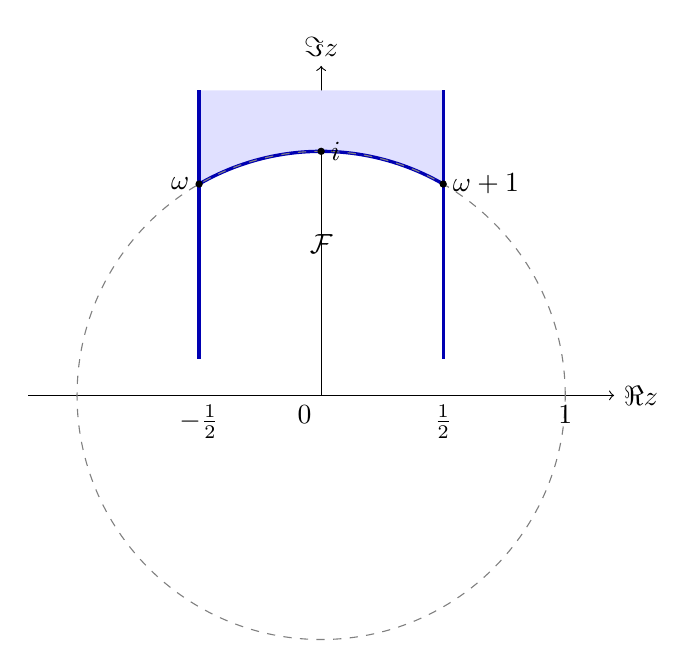
\begin{tikzpicture}[scale=3.1]
  % axes
  \draw[->, thin] (-1.2,0) -- (1.2,0) node[right] {$\Re z$};
  \draw[->, thin] (0,0) -- (0,1.35) node[above] {$\Im z$};

  % shaded region
  \fill[blue!12] (-0.5,1.25) -- (-0.5,0.8660254)
    arc[start angle=120,end angle=60,radius=1]
    -- (0.5,1.25) -- cycle;

  % boundaries
  \draw[very thick, blue!70!black] (-0.5,0.15) -- (-0.5,1.25);
  \draw[very thick, blue!70!black] (0.5,0.15) -- (0.5,1.25);
  \draw[very thick, blue!70!black] ({cos(120)},{sin(120)}) arc[start angle=120,end angle=60,radius=1];

  % dashed helper circle
  \draw[dashed, gray] (0,0) circle (1);

  % labels
  \fill (0,1) circle (0.015) node[right] {$i$};
  \fill (-0.5,0.8660254) circle (0.015) node[left] {$\omega$};
  \fill (0.5,0.8660254) circle (0.015) node[right] {$\omega+1$};
  \node at (0,0.62) {$\mathcal F$};
  \node[below] at (-0.5,0) {$-\frac12$};
  \node[below] at (0.5,0) {$\frac12$};
  \node[below left] at (0,0) {$0$};
  \node[below] at (1,0) {$1$};
\end{tikzpicture}
\caption{$\SL_2(\Z)$ 在上半平面上的标准基本域}
\end{figure}

\section{\texorpdfstring{$Y(\Gamma)$}{Y(Gamma)} 的直观理解}

本节只给出几何直观，不追求所有解析细节。真正严格的构造涉及复流形、黎曼曲面与局部坐标，但基本思想并不复杂：把 $\HH$ 中属于同一轨道的点识别起来，就得到一个新的几何对象。

\begin{definition}
设 $\Gamma\subseteq \SL_2(\Z)$ 是一个有限指标子群。记
\[
Y(\Gamma)=\Gamma\backslash \HH
\]
为其在 $\HH$ 上的商空间。
\end{definition}

\begin{remark}
直观上，$Y(\Gamma)$ 是把 $\HH$ 中所有由 $\Gamma$ 互相变换得到的点视为同一点所形成的空间。若 $\Gamma$ 没有有限阶非平凡元，则这个商空间局部看起来像开圆盘，因此是一个黎曼曲面；若有有限阶元，则会出现少数“锥点”，严格地说先得到一个一维复轨形（orbifold），但其底层拓扑空间仍可用黎曼曲面的语言描述。
\end{remark}

\begin{definition}
$\mathbf P^1(\Q)=\Q\cup\{\infty\}$ 上的点称为 $\Gamma$ 的\emph{尖点候选}。$\Gamma$ 对 $\mathbf P^1(\Q)$ 的作用同样由分式线性变换给出；其轨道称为 $\Gamma$ 的\emph{尖点}（cusps）。
\end{definition}

\begin{example}
对全模群 $\SL_2(\Z)$，所有有理点连同 $\infty$ 只形成一个尖点轨道。事实上，任意既约分数 $a/c$（$\gcd(a,c)=1$）都可由某个矩阵
\[
\mat{a&*\\ c&*}\in \SL_2(\Z)
\]
把 $\infty$ 送到 $a/c$。因此 $\SL_2(\Z)$ 只有一个尖点，通常记作 $\infty$。
\end{example}

\begin{remark}
尖点之所以要加入，是因为当 $\Im z\to\infty$ 时，点会“跑到无穷远处”。在商空间中，这种无穷远方向常常应被补上一个点。例如对 $\SL_2(\Z)$，在坐标
\[
q=e^{2\pi i z}
\]
下，$z\to i\infty$ 对应于 $q\to 0$，于是加入尖点等价于在 $q$-坐标中把原点补进去。
\end{remark}

\begin{definition}
把所有尖点加入 $Y(\Gamma)$，得到紧化空间
\[
X(\Gamma)=Y(\Gamma)\cup\{\text{尖点}\}.
\]
当 $\Gamma=\GammaO(N)$ 时，记
\[
Y_0(N)=\GammaO(N)\backslash \HH,
\qquad
X_0(N)=\GammaO(N)\backslash \HH^{\ast},
\]
其中 $\HH^{\ast}=\HH\cup \mathbf P^1(\Q)$。
\end{definition}

\begin{remark}
在模形式与椭圆曲线理论中，$Y_0(N)$ 具有非常重要的模解释：它参数化带有一个循环阶 $N$ 子群的椭圆曲线。换言之，$Y_0(N)$ 的点可以直观理解为“椭圆曲线加上一条 $N$-级结构”。紧化后的 $X_0(N)$ 则把退化情形（尖点）也纳入其中。
\end{remark}

\begin{theorem}[亏格公式，陈述]
设 $\Gamma\subseteq \SL_2(\Z)$ 是有限指标子群，记 $\bar\Gamma$ 为其在 $\PSL_2(\Z)$ 中的像，
\[
\mu=[\PSL_2(\Z):\bar\Gamma].
\]
再设 $\nu_2$、$\nu_3$ 分别为 $Y(\Gamma)$ 上椭圆点（稳定子阶分别为 $2$ 与 $3$）的个数，$\nu_{\infty}$ 为尖点个数。则紧化曲线 $X(\Gamma)$ 的亏格满足
\[
g\bigl(X(\Gamma)\bigr)=1+\frac{\mu}{12}-\frac{\nu_2}{4}-\frac{\nu_3}{3}-\frac{\nu_{\infty}}{2}.
\]
\end{theorem}

\begin{remark}
这条公式极其重要。它告诉我们：模曲线的拓扑复杂度（亏格）完全由有限个离散数据决定——指标、椭圆点个数、尖点个数。对于 $\GammaO(N)$，这些量都可以用算术方式计算，因此可以把一个高度几何的问题转化为纯代数与数论计算。
\end{remark}

\begin{example}
对 $\Gamma=\SL_2(\Z)$，有 $\mu=1$，$\nu_2=1$，$\nu_3=1$，$\nu_{\infty}=1$，故
\[
g\bigl(X(1)\bigr)=1+\frac1{12}-\frac14-\frac13-\frac12=0.
\]
因此 $X(1)$ 是亏格 $0$ 的曲线，事实上同构于复射影直线。这正是经典模 $j$-不变量出现的几何背景。
\end{example}

\section*{本章小结}

本章建立了模形式理论最核心的群论与几何背景：
\begin{itemize}
  \item $\GL_n(F)$ 与 $\SL_n(F)$ 通过行列式相联系；
  \item $\SL_2(\Z)$ 由 $S,T$ 两个基本矩阵生成；
  \item 合同子群 $\Gamma(N),\GammaO(N),\GammaI(N)$ 是研究不同级结构的自然对象；
  \item 群作用的轨道、稳定子与 Burnside 引理为“取商”提供了一般框架；
  \item $\SL_2(\Z)$ 通过 Möbius 变换作用在 $\HH$ 上，并拥有标准基本域；
  \item 模曲线 $Y(\Gamma)$ 与 $X(\Gamma)$ 是把上述群作用几何化后的产物。
\end{itemize}
后续章节中，模形式将作为这些群作用下满足特定变换律的解析函数出现，而本章给出的基本域、尖点与合同子群语言将反复使用。

\section*{习题}

下列习题按难度分为基础（\basic）、进阶（\medium）与挑战（\hard）三级，共 $65$ 题。建议先完成基础题，再做进阶题；挑战题适合在掌握本章主线后深入思考。

\subsection*{基础题（\basic）}

\begin{enumerate}
  \item[\basic 1.] 计算 $S^2$、$S^3$、$T^2$、$T^{-3}$，并验证它们都属于 $\SL_2(\Z)$。
  \item[\basic 2.] 直接计算 $ST$ 与 $TS$，并说明它们不相等。
  \item[\basic 3.] 设 $A=\mat{a&b\\ c&d}\in \SL_2(\Z)$。证明
  \[
  A^{-1}=\mat{d&-b\\ -c&a}.
  \]
  \item[\basic 4.] 对任意 $\lambda\in F^\times$，验证 $\operatorname{diag}(\lambda,1,\dots,1)\in \GL_n(F)$，且其行列式为 $\lambda$。
  \item[\basic 5.] 写出 $\GL_1(\F_5)$ 与 $\SL_1(\F_5)$ 的全部元素。
  \item[\basic 6.] 用列向量计数法计算 $|\GL_2(\F_2)|$。
  \item[\basic 7.] 用列向量计数法计算 $|\GL_2(\F_3)|$ 与 $|\SL_2(\F_3)|$。
  \item[\basic 8.] 证明 $\SL_n(F)$ 是 $\GL_n(F)$ 的正规子群。
  \item[\basic 9.] 说明 $\GL_n(\R)$ 中行列式为正的矩阵与行列式为负的矩阵不能落在同一个左陪集 $A\SL_n(\R)$ 中。
  \item[\basic 10.] 用 $S$ 的幂表示矩阵 $-I$。
  \item[\basic 11.] 直接验证关系 $(ST)^3=-I$。
  \item[\basic 12.] 计算 $ST^mS^{-1}$ 的显式矩阵形式，其中 $m\in\Z$。
  \item[\basic 13.] 证明 $\GammaO(2)$ 是 $\SL_2(\Z)$ 的子群。
  \item[\basic 14.] 判断下列矩阵分别是否属于 $\GammaO(3)$、$\GammaI(4)$、$\Gamma(5)$：
  \[
  \mat{1&2\\ 3&7},\qquad \mat{5&1\\ 4&1},\qquad \mat{6&5\\ 10&11}.
  \]
  \item[\basic 15.] 求矩阵 $\mat{7&4\\ 6&5}$ 在模 $3$ 与模 $5$ 下的约化像。
  \item[\basic 16.] 令循环群 $C_3$ 作用在正三角形的三个顶点上。求每个顶点的轨道与稳定子。
  \item[\basic 17.] 令正方形的对称群 $D_4$ 作用在四个顶点上。求某一固定顶点的稳定子大小。
  \item[\basic 18.] 对 $S_3$ 在集合 $\{1,2,3\}$ 上的自然作用，求 $\Orb(1)$ 与 $\Stab(1)$。
  \item[\basic 19.] 证明 $S$ 固定点 $i$，而 $T$ 在 $\HH$ 上没有不动点。
  \item[\basic 20.] 设 $z\in\HH$。证明
  \[
  \Im(z+1)=\Im z,
  \qquad
  \Im\!\left(-\frac1z\right)=\frac{\Im z}{|z|^2}.
  \]
  \item[\basic 21.] 把点 $2i$ 用 $\SL_2(\Z)$ 的作用化到基本域 $\mathcal F$ 中，并写出所用矩阵。
  \item[\basic 22.] 把点 $\frac{3+i}{2}$ 化到基本域 $\mathcal F$ 中。
  \item[\basic 23.] 证明 $0$ 与 $\infty$ 在 $\SL_2(\Z)$ 的作用下属于同一尖点轨道。
  \item[\basic 24.] 验证关系“$z\sim w$ 当且仅当存在 $\gamma\in\SL_2(\Z)$ 使 $w=\gamma\cdot z$”是等价关系。
  \item[\basic 25.] 设 $G$ 为有限群作用在有限集合 $X$ 上。证明对任意 $x\in X$，$\Stab(x)$ 是 $G$ 的子群。
\end{enumerate}

\subsection*{进阶题（\medium）}

\begin{enumerate}
  \item[\medium 26.] 设 $A=\mat{a&b\\ 1&d}\in \SL_2(\Z)$。利用本章中的归纳思想，把 $A$ 写成 $S$ 与 $T$ 的乘积。
  \item[\medium 27.] 完整证明：若
  \[
  A=\mat{a&b\\ c&d}\in \SL_2(\Z),
  \]
  则存在整数 $q$ 使得 $ST^{-q}A$ 的左下角绝对值严格小于 $|c|$。
  \item[\medium 28.] 证明 $\bar S,\bar T$ 生成 $\SL_2(\Z/2\Z)$。
  \item[\medium 29.] 证明 $\bar S,\bar T$ 生成 $\SL_2(\Z/3\Z)$。
  \item[\medium 30.] 证明模 $N$ 约化映射 $\rho_N$ 的核恰为 $\Gamma(N)$。
  \item[\medium 31.] 证明 $\Gamma(N)$ 是 $\SL_2(\Z)$ 的正规子群。
  \item[\medium 32.] 用指标公式计算 $[\SL_2(\Z):\GammaO(2)]$。
  \item[\medium 33.] 用指标公式计算 $[\SL_2(\Z):\GammaO(3)]$。
  \item[\medium 34.] 用指标公式计算 $[\SL_2(\Z):\GammaO(4)]$。
  \item[\medium 35.] 用指标公式计算 $[\SL_2(\Z):\GammaO(6)]$。
  \item[\medium 36.] 证明
  \[
  [\SL_2(\Z):\GammaI(5)]=24.
  \]
  \item[\medium 37.] 证明一般公式
  \[
  [\GammaO(N):\GammaI(N)]=\varphi(N).
  \]
  \item[\medium 38.] 利用 Burnside 引理证明：若素数阶循环群 $C_p$ 作用在有限集合 $X$ 上，则
  \[
  |X|\equiv |\Fix(C_p)|\pmod p,
  \]
  其中 $\Fix(C_p)$ 表示被所有群元素固定的点集。
  \item[\medium 39.] 研究 $\SL_2(\Z)$ 对原始整数向量集
  \[
  \{(m,n)\in\Z^2:\gcd(m,n)=1\}
  \]
  的作用，证明该作用是传递的。
  \item[\medium 40.] 证明对任意 $z\in\HH$，存在整数 $n$ 使得 $|\Re(z+n)|\le 1/2$。
  \item[\medium 41.] 设 $w\in\HH$ 且 $|\Re w|\le 1/2$。证明若 $|w|<1$，则 $\Im(S\cdot w)>\Im w$。
  \item[\medium 42.] 结合前两题，重新证明每个 $z\in\HH$ 都与基本域 $\mathcal F$ 中某点等价。
  \item[\medium 43.] 证明：若 $z,w\in\mathcal F^\circ$ 且 $w=\gamma\cdot z$，则 $z=w$。
  \item[\medium 44.] 详细说明基本域 $\mathcal F$ 两侧边界与圆弧边界分别由哪些群元素配对。
  \item[\medium 45.] 在 $\PSL_2(\Z)$ 中，证明点 $i$ 的稳定子阶为 $2$，点 $\omega$ 的稳定子阶为 $3$。
  \item[\medium 46.] 求由子群 $\langle T\rangle$ 在 $\HH$ 上作用的一个基本域，并证明你的答案正确。
  \item[\medium 47.] 求由子群 $\langle T^2\rangle$ 在 $\HH$ 上作用的一个基本域，并与上一题比较。
  \item[\medium 48.] 用 $\mathbf{P}^1(\Z/N\Z)$ 上的群作用，重新推导
  \[
  [\SL_2(\Z):\GammaO(N)]
  =N\prod_{p\mid N}\left(1+\frac1p\right).
  \]
  \item[\medium 49.] 计算 $\bigl|\mathbf{P}^1(\Z/8\Z)\bigr|$，并由此求 $[\SL_2(\Z):\GammaO(8)]$。
  \item[\medium 50.] 查阅或自行构造 $\GammaO(2)$ 与 $\GammaO(3)$ 在 $\HH$ 上的基本域草图，并说明它们为何应由有限个 $\SL_2(\Z)$ 标准基本域拼接而成。
\end{enumerate}

\subsection*{挑战题（\hard）}

\begin{enumerate}
  \item[\hard 51.] 设
  \[
  \mathcal M=\left\{z\mapsto \frac{az+b}{cz+d}:a,b,c,d\in\R,\ ad-bc\ne 0\right\}.
  \]
  证明在复合运算下，$\mathcal M$ 形成一个群，并说明它与适当的矩阵商群同构。
  \item[\hard 52.] 证明 $\SL_2(\R)$ 在 $\HH$ 上的作用通过 $\PSL_2(\R)$ 因子化，并讨论为何标量矩阵不改变 Möbius 变换。
  \item[\hard 53.] 设 $\gamma\in\SL_2(\Z)$。证明：$\gamma$ 在 $\HH$ 中有不动点当且仅当 $|\operatorname{tr}(\gamma)|<2$。
  \item[\hard 54.] 证明 $\SL_2(\Z)$ 中每个有限阶非平凡元素都共轭于 $S$ 或 $ST$（在 $\PSL_2(\Z)$ 中分别对应阶 $2$ 与阶 $3$ 的元素）。
  \item[\hard 55.] 证明 $\GammaO(N)$ 的每个尖点都可由某个有理数 $a/c$ 表示，其中 $c\mid N$。
  \item[\hard 56.] 证明 $\GammaO(N)$ 的尖点个数公式
  \[
  \nu_{\infty}(N)=\sum_{d\mid N}\varphi\bigl(\gcd(d,N/d)\bigr).
  \]
  \item[\hard 57.] 利用上一题的公式，求 $\GammaO(11)$ 的尖点个数，并给出一组代表元。
  \item[\hard 58.] 通过对基本域作三角剖分，推导亏格公式
  \[
  g=1+\frac{\mu}{12}-\frac{\nu_2}{4}-\frac{\nu_3}{3}-\frac{\nu_{\infty}}{2}.
  \]
  \item[\hard 59.] 利用指标、椭圆点与尖点数据，计算 $X_0(11)$ 的亏格。
  \item[\hard 60.] 证明并讨论：对哪些 $N$，曲线 $X_0(N)$ 没有来自 $i$ 的椭圆点（即没有阶 $2$ 椭圆点）？
  \item[\hard 61.] 证明并讨论：对哪些 $N$，曲线 $X_0(N)$ 没有来自 $\omega$ 的椭圆点（即没有阶 $3$ 椭圆点）？
  \item[\hard 62.] 研究 $\SL_2(\F_3)$ 对射影直线 $\mathbf P^1(\F_3)$ 的作用，证明其传递性并求稳定子大小。
  \item[\hard 63.] 不借助本章推论，直接从定义出发证明
  \[
  |\SL_2(\F_q)|=q(q^2-1).
  \]
  \item[\hard 64.] 证明主合同子群 $\Gamma(N)$ 在 $N\ge 3$ 时无非平凡有限阶元；换言之，$\Gamma(N)$ 是无挠群。
  \item[\hard 65.] 证明
  \[
  \PSL_2(\Z)\cong C_2\ast C_3,
  \]
  即它同构于一个阶 $2$ 循环群与一个阶 $3$ 循环群的自由积。
\end{enumerate}

\section*{习题解答}
\begin{enumerate}[label=\textbf{\arabic*.}, leftmargin=*, itemsep=1em]
\item \textbf{解答.} 由
\[
S=\mat{0&-1\\ 1&0},\qquad T=\mat{1&1\\ 0&1}
\]
直接计算得
\[
S^2=\mat{-1&0\\ 0&-1}=-I,\qquad
S^3=S^2S=\mat{0&1\\ -1&0},
\]
\[
T^2=\mat{1&2\\ 0&1},\qquad
T^{-3}=\mat{1&-3\\ 0&1}.
\]
又
\[
\det(S^2)=\det(S^3)=\det(T^2)=\det(T^{-3})=1,
\]
且各矩阵条目都在 $\Z$ 中，所以它们都属于 $\SL_2(\Z)$。

\item \textbf{解答.} 有
\[
ST=\mat{0&-1\\ 1&0}\mat{1&1\\ 0&1}
=\mat{0&-1\\ 1&1},
\]
\[
TS=\mat{1&1\\ 0&1}\mat{0&-1\\ 1&0}
=\mat{1&-1\\ 1&0}.
\]
因此
\[
ST\neq TS.
\]

\item \textbf{解答.} 设
\[
A=\mat{a&b\\ c&d}\in \SL_2(\Z),
\]
则 $\det A=ad-bc=1$。于是
\[
A\mat{d&-b\\ -c&a}
=\mat{ad-bc&-ab+ab\\ cd-dc&-cb+ad}
=\mat{1&0\\ 0&1}=I.
\]
同理
\[
\mat{d&-b\\ -c&a}A=I.
\]
故
\[
A^{-1}=\mat{d&-b\\ -c&a}.
\]

\item \textbf{解答.} 令
\[
D=\operatorname{diag}(\lambda,1,\dots,1),\qquad \lambda\in F^\times.
\]
则
\[
D^{-1}=\operatorname{diag}(\lambda^{-1},1,\dots,1),
\]
所以 $D\in \GL_n(F)$。对角矩阵的行列式等于对角元之积，故
\[
\det D=\lambda\cdot 1\cdots 1=\lambda.
\]

\item \textbf{解答.} 由定义
\[
\GL_1(\F_5)=\F_5^\times=\{1,2,3,4\}.
\]
而 $\SL_1(\F_5)$ 由行列式等于 $1$ 的 $1\times1$ 矩阵组成，因此
\[
\SL_1(\F_5)=\{1\}.
\]

\item \textbf{解答.} 在 $\F_2^2$ 中，可逆矩阵的两列必须线性无关。第一列可任取非零向量，共
\[
2^2-1=3
\]
种。取定第一列后，第二列不能落在它张成的一维子空间中；该子空间有 $2$ 个向量，所以第二列有
\[
2^2-2=2
\]
种。故
\[
|\GL_2(\F_2)|=3\cdot 2=6.
\]

\item \textbf{解答.} 同理，在 $\F_3^2$ 中，第一列有
\[
3^2-1=8
\]
种非零选法。第二列不能在第一列张成的直线中；该直线有 $3$ 个向量，所以第二列有
\[
3^2-3=6
\]
种。故
\[
|\GL_2(\F_3)|=8\cdot 6=48.
\]
行列式映射
\[
\det:\GL_2(\F_3)\to \F_3^\times
\]
满射，而 $|\F_3^\times|=2$，其核为 $\SL_2(\F_3)$，所以
\[
|\SL_2(\F_3)|=\frac{48}{2}=24.
\]

\item \textbf{解答.} 行列式给出群同态
\[
\det:\GL_n(F)\longrightarrow F^\times.
\]
由定义
\[
\SL_n(F)=\{A\in \GL_n(F):\det A=1\}=\ker(\det).
\]
群同态的核总是正规子群，故
\[
\SL_n(F)\trianglelefteq \GL_n(F).
\]

\item \textbf{解答.} 固定 $A\in \GL_n(\R)$。若 $B\in A\SL_n(\R)$，则可写成 $B=AM$，其中 $M\in \SL_n(\R)$，故
\[
\det B=\det A\det M=\det A.
\]
因此同一个左陪集 $A\SL_n(\R)$ 中所有矩阵的行列式都与 $\det A$ 相同，特别具有相同符号。故行列式为正的矩阵与行列式为负的矩阵不可能落在同一左陪集里。

\item \textbf{解答.} 由
\[
S^2=-I,
\]
故
\[
-I=S^2.
\]

\item \textbf{解答.} 先算
\[
ST=\mat{0&-1\\ 1&1}.
\]
于是
\[
(ST)^2=\mat{0&-1\\ 1&1}\mat{0&-1\\ 1&1}
=\mat{-1&-1\\ 1&0},
\]
再乘一次得
\[
(ST)^3=\mat{-1&-1\\ 1&0}\mat{0&-1\\ 1&1}
=\mat{-1&0\\ 0&-1}=-I.
\]

\item \textbf{解答.} 由
\[
T^m=\mat{1&m\\ 0&1},\qquad S^{-1}=-S=\mat{0&1\\ -1&0},
\]
得
\[
ST^m=\mat{0&-1\\ 1&0}\mat{1&m\\ 0&1}
=\mat{0&-1\\ 1&m},
\]
故
\[
ST^mS^{-1}
=\mat{0&-1\\ 1&m}\mat{0&1\\ -1&0}
=\mat{1&0\\ -m&1}.
\]

\item \textbf{解答.} 记
\[
\GammaO(2)=\left\{\mat{a&b\\ c&d}\in \SL_2(\Z):c\equiv 0\pmod 2\right\}.
\]
单位元 $I$ 显然在其中。若
\[
A=\mat{a&b\\ c&d},\qquad B=\mat{a'&b'\\ c'&d'}\in \GammaO(2),
\]
则
\[
AB=\mat{aa'+bc'&ab'+bd'\\ ca'+dc'&cb'+dd'},
\]
其左下角为 $ca'+dc'$，仍被 $2$ 整除，所以 $AB\in\GammaO(2)$。又
\[
A^{-1}=\mat{d&-b\\ -c&a},
\]
其左下角为 $-c$，仍被 $2$ 整除，所以 $A^{-1}\in\GammaO(2)$。故 $\GammaO(2)$ 是 $\SL_2(\Z)$ 的子群。

\item \textbf{解答.} 先算行列式：
\[
\det\mat{1&2\\ 3&7}=1,\qquad
\det\mat{5&1\\ 4&1}=1,\qquad
\det\mat{6&5\\ 10&11}=16\neq 1.
\]
所以第三个矩阵不在 $\SL_2(\Z)$，因而不属于 $\GammaO(3),\GammaI(4),\Gamma(5)$ 中的任何一个。

对第一个矩阵 $\mat{1&2\\ 3&7}$，有 $c=3\equiv0\pmod 3$，故属于 $\GammaO(3)$；但
\[
c=3\not\equiv 0\pmod 4,
\]
故不属于 $\GammaI(4)$；又它模 $5$ 不与 $I$ 同余，故不属于 $\Gamma(5)$。

对第二个矩阵 $\mat{5&1\\ 4&1}$，有
\[
c=4\not\equiv0\pmod 3,
\]
故不属于 $\GammaO(3)$；而
\[
a=5\equiv1,\quad d=1\equiv1,\quad c=4\equiv0\pmod 4,
\]
故属于 $\GammaI(4)$；又 $a=5\equiv0\not\equiv1\pmod 5$，故不属于 $\Gamma(5)$。

综上，
\[
\mat{1&2\\ 3&7}\in \GammaO(3),\ \notin \GammaI(4),\ \notin \Gamma(5),
\]
\[
\mat{5&1\\ 4&1}\notin \GammaO(3),\ \in \GammaI(4),\ \notin \Gamma(5),
\]
\[
\mat{6&5\\ 10&11}\notin \GammaO(3),\ \notin \GammaI(4),\ \notin \Gamma(5).
\]

\item \textbf{解答.} 逐项模约化得
\[
\mat{7&4\\ 6&5}\equiv \mat{1&1\\ 0&2}\pmod 3,
\qquad
\mat{7&4\\ 6&5}\equiv \mat{2&4\\ 1&0}\pmod 5.
\]

\item \textbf{解答.} 设正三角形顶点为 $v_1,v_2,v_3$，群 $C_3=\langle r\rangle$ 由 $120^\circ$ 旋转生成。旋转可把任一顶点送到任一顶点，所以对每个顶点
\[
\Orb(v_i)=\{v_1,v_2,v_3\}.
\]
若 $r^k$ 固定某个顶点，则旋转角只能是 $0^\circ$，故 $r^k=e$。因此
\[
\Stab(v_i)=\{e\}.
\]

\item \textbf{解答.} 固定一个顶点 $v$。在 $D_4$ 中能固定 $v$ 的对称只有两个：恒等变换，以及经过 $v$ 与对角顶点所连对角线的反射。其余旋转和反射都会移动 $v$。故
\[
|\Stab(v)|=2.
\]

\item \textbf{解答.} 在自然作用下，$S_3$ 可把 $1$ 送到 $1,2,3$ 中任意一点，所以
\[
\Orb(1)=\{1,2,3\}.
\]
稳定子由所有固定 $1$ 的置换组成，只能在 $\{2,3\}$ 上作置换，因此
\[
\Stab(1)=\{\Id,(23)\}.
\]

\item \textbf{解答.} 由作用公式，
\[
S\cdot i=\frac{0\cdot i-1}{1\cdot i+0}=-\frac1i=i,
\]
故 $S$ 固定点 $i$。

而
\[
T\cdot z=z+1.
\]
若 $T$ 在 $\HH$ 上有不动点 $z$，则 $z+1=z$，矛盾。所以 $T$ 在 $\HH$ 上没有不动点。

\item \textbf{解答.} 设 $z=x+iy\in\HH$，其中 $y>0$。则
\[
z+1=(x+1)+iy,
\]
故
\[
\Im(z+1)=y=\Im z.
\]
又
\[
-\frac1z=-\frac{x-iy}{x^2+y^2}=\frac{-x+iy}{x^2+y^2},
\]
因此
\[
\Im\!\left(-\frac1z\right)=\frac{y}{x^2+y^2}
=\frac{\Im z}{|z|^2}.
\]

\item \textbf{解答.} 点 $2i$ 满足
\[
|2i|=2\ge 1,\qquad |\Re(2i)|=0\le \frac12,
\]
所以 $2i\in\mathcal F$。因此可取所用矩阵为单位矩阵
\[
I=\mat{1&0\\ 0&1},
\]
并有
\[
I\cdot 2i=2i.
\]

\item \textbf{解答.} 设
\[
z=\frac{3+i}{2}.
\]
先用 $T^{-1}$：
\[
T^{-1}\cdot z=z-1=\frac{1+i}{2}.
\]
此时
\[
\left|\frac{1+i}{2}\right|=\frac1{\sqrt2}<1.
\]
再用 $S$：
\[
S\cdot \frac{1+i}{2}=-\frac{1}{(1+i)/2}=-1+i.
\]
最后用 $T$：
\[
T\cdot(-1+i)=i.
\]
而 $i\in\mathcal F$，故所求矩阵可取
\[
\gamma=TST^{-1}=\mat{1&-2\\ 1&-1},
\]
并且
\[
\gamma\cdot \frac{3+i}{2}=i.
\]

\item \textbf{解答.} 矩阵
\[
S=\mat{0&-1\\ 1&0}
\]
作用为
\[
S\cdot z=-\frac1z.
\]
在尖点上延拓后，
\[
S\cdot \infty=0,\qquad S\cdot 0=\infty.
\]
故 $0$ 与 $\infty$ 属于同一 $\SL_2(\Z)$-轨道，也就是同一尖点。

\item \textbf{解答.} 记
\[
z\sim w \iff \exists\,\gamma\in\SL_2(\Z)\ \text{使}\ w=\gamma\cdot z.
\]
验证三条性质：

反身性：取 $\gamma=I$，则 $z=I\cdot z$，故 $z\sim z$。

对称性：若 $w=\gamma\cdot z$，则
\[
z=\gamma^{-1}\cdot w,
\]
且 $\gamma^{-1}\in\SL_2(\Z)$，故 $w\sim z$。

传递性：若 $w=\gamma_1\cdot z$ 且 $u=\gamma_2\cdot w$，则
\[
u=\gamma_2\cdot(\gamma_1\cdot z)=(\gamma_2\gamma_1)\cdot z,
\]
而 $\gamma_2\gamma_1\in\SL_2(\Z)$，故 $z\sim u$。

所以 $\sim$ 是等价关系。

\item \textbf{解答.} 定义
\[
\Stab(x)=\{g\in G:g\cdot x=x\}.
\]
先有
\[
\Id\cdot x=x,
\]
故 $\Id\in\Stab(x)$。若 $g,h\in\Stab(x)$，则
\[
(gh)\cdot x=g\cdot(h\cdot x)=g\cdot x=x,
\]
所以 $gh\in\Stab(x)$。若 $g\in\Stab(x)$，则 $g\cdot x=x$，两边左乘 $g^{-1}$ 得
\[
g^{-1}\cdot x=x,
\]
故 $g^{-1}\in\Stab(x)$。因此 $\Stab(x)$ 是 $G$ 的子群。

\item \textbf{解答.} 由
\[
A=\mat{a&b\\ 1&d}\in\SL_2(\Z)
\]
知
\[
ad-b=1\quad\Longrightarrow\quad b=ad-1.
\]
而
\[
T^aST^d
=\mat{1&a\\ 0&1}\mat{0&-1\\ 1&0}\mat{1&d\\ 0&1}
=\mat{a&ad-1\\ 1&d}.
\]
因此
\[
A=T^aST^d.
\]

\item \textbf{解答.} 设
\[
A=\mat{a&b\\ c&d}\in\SL_2(\Z),\qquad c\neq 0.
\]
对任意整数 $q$，
\[
T^{-q}A=\mat{a-qc&b-qd\\ c&d},
\]
从而
\[
ST^{-q}A=\mat{-c&-d\\ a-qc&b-qd}.
\]
所以 $ST^{-q}A$ 的左下角就是 $a-qc$。由整数除法，可取 $q\in\Z$ 使
\[
\left|\frac ac-q\right|\le \frac12.
\]
于是
\[
|a-qc|=|c|\left|\frac ac-q\right|\le \frac{|c|}{2}<|c|.
\]
这就证明了存在这样的整数 $q$。

\item \textbf{解答.} 因为 $\SL_2(\Z)$ 由 $S,T$ 生成，而模 $2$ 约化映射
\[
\rho_2:\SL_2(\Z)\to \SL_2(\Z/2\Z)
\]
是满射，所以 $\SL_2(\Z/2\Z)$ 由 $\bar S=\rho_2(S)$ 与 $\bar T=\rho_2(T)$ 生成。

若要直接看，也可算出
\[
|\SL_2(\Z/2\Z)|=|\GL_2(\F_2)|=6,
\]
而由 $\bar S,\bar T$ 可得到 $I,\bar S,\bar T,\bar S\bar T,\bar T\bar S,\bar S\bar T\bar S$ 六个不同元素，故它们确实生成整个群。

\item \textbf{解答.} 同理，由 $\SL_2(\Z)=\langle S,T\rangle$ 且
\[
\rho_3:\SL_2(\Z)\to \SL_2(\Z/3\Z)
\]
是满射，立刻得到 $\SL_2(\Z/3\Z)$ 由 $\bar S,\bar T$ 生成。

\item \textbf{解答.} 由定义，
\[
\rho_N\!\left(\mat{a&b\\ c&d}\right)=\mat{\bar a&\bar b\\ \bar c&\bar d}.
\]
因此
\[
A\in\ker(\rho_N)
\iff \bar a=\bar d=1,\ \bar b=\bar c=0
\iff A\equiv I\pmod N.
\]
而这正是 $\Gamma(N)$ 的定义，所以
\[
\ker(\rho_N)=\Gamma(N).
\]

\item \textbf{解答.} 由上一题，
\[
\Gamma(N)=\ker(\rho_N).
\]
群同态的核总是正规子群，故
\[
\Gamma(N)\trianglelefteq \SL_2(\Z).
\]

\item \textbf{解答.} 指标公式给出
\[
[\SL_2(\Z):\GammaO(N)]
=N\prod_{p\mid N}\left(1+\frac1p\right).
\]
当 $N=2$ 时，
\[
[\SL_2(\Z):\GammaO(2)]
=2\left(1+\frac12\right)=3.
\]

\item \textbf{解答.} 由指标公式，
\[
[\SL_2(\Z):\GammaO(3)]
=3\left(1+\frac13\right)=4.
\]

\item \textbf{解答.} 由指标公式，
\[
[\SL_2(\Z):\GammaO(4)]
=4\left(1+\frac12\right)=6.
\]

\item \textbf{解答.} 因为 $6=2\cdot 3$，故
\[
[\SL_2(\Z):\GammaO(6)]
=6\left(1+\frac12\right)\left(1+\frac13\right)
=6\cdot \frac32\cdot \frac43=12.
\]

\item \textbf{解答.} 由公式
\[
[\SL_2(\Z):\GammaI(N)]
=N^2\prod_{p\mid N}\left(1-\frac1{p^2}\right),
\]
取 $N=5$ 得
\[
[\SL_2(\Z):\GammaI(5)]
=25\left(1-\frac1{25}\right)=24.
\]

\item \textbf{解答.} 考虑群同态
\[
\GammaO(N)\longrightarrow (\Z/N\Z)^\times,\qquad
\mat{a&b\\ c&d}\longmapsto \bar a.
\]
因为在 $\GammaO(N)$ 中有 $c\equiv 0\pmod N$ 且 $ad-bc=1$，故
\[
\bar a\,\bar d=1,
\]
所以 $\bar a\in(\Z/N\Z)^\times$。其核恰为满足
\[
a\equiv d\equiv 1,\qquad c\equiv 0\pmod N
\]
的矩阵，即 $\GammaI(N)$。该映射满射，因此
\[
[\GammaO(N):\GammaI(N)]
=|(\Z/N\Z)^\times|
=\varphi(N).
\]

\item \textbf{解答.} 设 $G=C_p$，轨道个数为 $r$。对任意非单位元 $g\in C_p$，它固定的点恰是被整个 $C_p$ 固定的点，因此
\[
|\Fix(g)|=|\Fix(C_p)|\qquad (g\neq 1).
\]
由 Burnside 引理，
\[
r=\frac1p\Bigl(|X|+(p-1)|\Fix(C_p)|\Bigr).
\]
右边必须是整数，所以
\[
|X|+(p-1)|\Fix(C_p)|\equiv 0\pmod p.
\]
即
\[
|X|-|\Fix(C_p)|\equiv 0\pmod p,
\]
故
\[
|X|\equiv |\Fix(C_p)|\pmod p.
\]

\item \textbf{解答.} 设
\[
X=\{(m,n)\in\Z^2:\gcd(m,n)=1\}.
\]
取任意 $(m,n)\in X$。由 Bézout 等式，存在整数 $x,y$ 使
\[
my-nx=1.
\]
于是
\[
A=\mat{m&x\\ n&y}\in \SL_2(\Z),
\]
并且
\[
A\binom10=\binom mn.
\]
因此每个原始向量都在 $(1,0)^t$ 的轨道中，即该作用是传递的。

\item \textbf{解答.} 设 $z=x+iy$。取整数 $n$ 为最接近 $-x$ 的整数，则
\[
|x+n|\le \frac12.
\]
而
\[
\Re(z+n)=x+n,
\]
所以
\[
|\Re(z+n)|\le \frac12.
\]

\item \textbf{解答.} 由
\[
S\cdot w=-\frac1w
\]
以及虚部变换公式，
\[
\Im(S\cdot w)=\frac{\Im w}{|w|^2}.
\]
若 $|w|<1$，则 $1/|w|^2>1$，故
\[
\Im(S\cdot w)=\frac{\Im w}{|w|^2}>\Im w.
\]

\item \textbf{解答.} 给定 $z\in\HH$。在其 $\SL_2(\Z)$-轨道中取虚部最大的点 $w$。由上一题，可再取整数 $n$，使
\[
|\Re(w+n)|\le \frac12.
\]
因为 $T^n$ 不改变虚部，所以仍可记该点为 $w$，并有
\[
|\Re w|\le \frac12.
\]
若 $|w|<1$，则由上一题
\[
\Im(S\cdot w)>\Im w,
\]
与 $w$ 的虚部最大矛盾。故必有 $|w|\ge 1$。于是
\[
w\in\mathcal F.
\]
所以每个 $z\in\HH$ 都与 $\mathcal F$ 中某点等价。

\item \textbf{解答.} 设
\[
z,w\in\mathcal F^\circ,\qquad w=\gamma\cdot z,\qquad \gamma=\mat{a&b\\ c&d}.
\]
由本章定理，只要 $z\in\mathcal F^\circ$，若 $(c,d)\neq(0,\pm1)$，便有
\[
|cz+d|>1.
\]
于是
\[
\Im w=\frac{\Im z}{|cz+d|^2}<\Im z.
\]
把同样论证应用于 $\gamma^{-1}$，又得 $\Im z<\Im w$，矛盾。故只可能
\[
c=0,\qquad d=\pm1.
\]
再由 $\det\gamma=1$ 得 $a=d=\pm1$，故
\[
\gamma=\pm\mat{1&n\\ 0&1}
\]
对某个 $n\in\Z$。在 $\HH$ 上 $-I$ 作用平凡，所以
\[
w=z+n.
\]
但 $z,w\in\mathcal F^\circ$ 都满足 $|\Re|<1/2$，只能有 $n=0$，故
\[
w=z.
\]

\item \textbf{解答.} 标准基本域
\[
\mathcal F=\left\{z\in\HH:|z|\ge1,\ |\Re z|\le \frac12\right\}
\]
有两类边界配对：

其一，竖边
\[
\Re z=-\frac12\quad\text{与}\quad \Re z=\frac12
\]
由平移
\[
T:z\mapsto z+1
\]
配对，因为
\[
T\cdot\left(-\frac12+iy\right)=\frac12+iy.
\]

其二，圆弧边界
\[
|z|=1,\qquad -\frac12\le \Re z\le \frac12
\]
由
\[
S:z\mapsto -\frac1z
\]
配对；当 $|z|=1$ 时，
\[
S\cdot z=-\frac1z=-\bar z,
\]
它把圆弧左半边送到右半边，右半边送到左半边。

特殊点中，
\[
S\cdot i=i,
\]
所以 $i$ 是阶 $2$ 椭圆点；两端点
\[
\omega=\frac{-1+\sqrt3\,i}{2},\qquad \omega+1=\frac{1+\sqrt3\,i}{2}
\]
分别落在两侧竖边上，由 $T$ 识别，而 $\omega$ 又满足 $(ST)\cdot\omega=\omega$。

\item \textbf{解答.} 先看 $i$。由
\[
S\cdot i=i
\]
知 $\bar S$ 在 $\PSL_2(\Z)$ 中属于 $\Stab(i)$。又 $\bar S^2=\Id$，所以它给出一个阶 $2$ 元。若 $\bar\gamma\in\PSL_2(\Z)$ 也固定 $i$，则它是有限阶元；而标准基本域中通过 $i$ 的唯一非平凡边识别来自 $S$，故
\[
\Stab(i)=\{1,\bar S\},
\]
其阶为 $2$。

再看
\[
\omega=e^{2\pi i/3}=\frac{-1+\sqrt3\,i}{2}.
\]
由
\[
(ST)\cdot\omega=\omega,\qquad (\overline{ST})^3=\Id
\]
知 $\overline{ST}\in\Stab(\omega)$ 且其阶为 $3$。标准基本域中通过 $\omega$ 的非平凡识别正对应三块小三角形绕点拼接，因此
\[
\Stab(\omega)=\{1,\overline{ST},\overline{(ST)^2}\},
\]
其阶为 $3$。

\item \textbf{解答.} 因为
\[
T:z\mapsto z+1,
\]
所以可取竖条带
\[
D=\{z\in\HH:0\le \Re z<1\}
\]
为 $\langle T\rangle$ 的一个基本域。确实，对任意 $z=x+iy\in\HH$，存在唯一整数 $n$ 使
\[
x-n\in[0,1),
\]
从而
\[
T^{-n}\cdot z=z-n\in D.
\]
若 $z,z'\in D$ 且 $z'=T^m\cdot z=z+m$，则两点实部都在 $[0,1)$ 中，只能有 $m=0$。故该表示唯一，所以 $D$ 是基本域。

\item \textbf{解答.} 因为
\[
T^2:z\mapsto z+2,
\]
故可取
\[
D_2=\{z\in\HH:0\le \Re z<2\}
\]
为 $\langle T^2\rangle$ 的一个基本域。证明与上一题相同：任意点可唯一平移入该条带。

与上一题比较，$\langle T^2\rangle$ 在 $\langle T\rangle$ 中指数为 $2$，所以其基本域正好可看成上一题基本域的两个相邻副本之并：
\[
D_2=D\cup T\cdot D.
\]

\item \textbf{解答.} 约化映射
\[
\rho_N:\SL_2(\Z)\to \SL_2(\Z/N\Z)
\]
满射，且 $\GammaO(N)$ 的像正是 $\SL_2(\Z/N\Z)$ 在 $\mathbf P^1(\Z/N\Z)$ 上固定点 $[1:0]$ 的稳定子：因为
\[
\mat{a&b\\ c&d}\binom10=\binom ac,
\]
固定 $[1:0]$ 当且仅当 $c\equiv0\pmod N$。故
\[
[\SL_2(\Z):\GammaO(N)]
=[\SL_2(\Z/N\Z):\Stab([1:0])]
=\bigl|\mathbf P^1(\Z/N\Z)\bigr|.
\]
若 $N=p^r$，则
\[
\bigl|\mathbf P^1(\Z/p^r\Z)\bigr|=p^r+p^{r-1}=p^r\left(1+\frac1p\right).
\]
再由中国剩余定理的乘法性，
\[
\bigl|\mathbf P^1(\Z/N\Z)\bigr|
=N\prod_{p\mid N}\left(1+\frac1p\right).
\]
于是
\[
[\SL_2(\Z):\GammaO(N)]
=N\prod_{p\mid N}\left(1+\frac1p\right).
\]

\item \textbf{解答.} 因为 $8=2^3$，所以
\[
\bigl|\mathbf P^1(\Z/8\Z)\bigr|
=2^3+2^2=8+4=12.
\]
因此
\[
[\SL_2(\Z):\GammaO(8)]=12.
\]

\item \textbf{解答.} 因为 $\GammaO(N)$ 在 $\SL_2(\Z)$ 中是有限指标子群，设
\[
[\SL_2(\Z):\GammaO(N)]=r,
\]
取一组左陪集代表 $\gamma_1,\dots,\gamma_r$，则
\[
\gamma_1\mathcal F,\dots,\gamma_r\mathcal F
\]
的并经边界适当识别后给出 $\GammaO(N)$ 的一个基本域。所以它必由有限个 $\SL_2(\Z)$ 的标准基本域拼接而成。

对 $N=2$，指标为
\[
[\SL_2(\Z):\GammaO(2)]=3,
\]
故基本域可由 $3$ 个标准基本域拼接而成；例如可取陪集代表
\[
I,\ S,\ TS.
\]

对 $N=3$，指标为
\[
[\SL_2(\Z):\GammaO(3)]=4,
\]
故基本域可由 $4$ 个标准基本域拼接而成；例如可取陪集代表
\[
I,\ S,\ TS,\ T^{-1}S.
\]
把这些像沿公共边拼接，就得到常见的 $\GammaO(2)$ 与 $\GammaO(3)$ 基本域草图。

\item \textbf{解答.} 设
\[
T_A(z)=\frac{az+b}{cz+d}\qquad \left(A=\mat{a&b\\ c&d},\ \det A\neq0\right).
\]
则
\[
T_A\circ T_B=T_{AB},
\]
所以闭合性与结合律都来自矩阵乘法。单位元是
\[
T_I(z)=z.
\]
若 $\det A\neq0$，则
\[
T_A^{-1}=T_{A^{-1}},
\]
故每个元素都可逆，因此 $\mathcal M$ 在复合下成群。

再定义
\[
\Phi:\GL_2(\R)\to\mathcal M,\qquad A\mapsto T_A.
\]
这是满同态，且
\[
T_{\lambda A}=T_A\qquad (\lambda\in\R^\times).
\]
反之，若 $T_A=T_B$，则
\[
\frac{az+b}{cz+d}=\frac{a'z+b'}{c'z+d'}
\]
对所有 $z$ 成立，交叉相乘比较系数可得 $B=\lambda A$。故
\[
\ker\Phi=\R^\times I.
\]
因此
\[
\mathcal M\cong \GL_2(\R)/\R^\times I=\PGL_2(\R).
\]

\item \textbf{解答.} 对
\[
A=\mat{a&b\\ c&d}\in\SL_2(\R),
\]
作用定义为
\[
A\cdot z=\frac{az+b}{cz+d}.
\]
若 $\lambda\neq0$，则
\[
\frac{\lambda az+\lambda b}{\lambda cz+\lambda d}=\frac{az+b}{cz+d},
\]
故非零标量倍给出同一个 Möbius 变换。特别地，在 $\SL_2(\R)$ 中只有 $\pm I$ 是标量矩阵，而
\[
(-I)\cdot z=z.
\]
因此该作用的核恰为 $\{\pm I\}$，从而它通过商群
\[
\PSL_2(\R)=\SL_2(\R)/\{\pm I\}
\]
因子化。

\item \textbf{解答.} 严格地说，本章命题的结论对 $\gamma\neq\pm I$ 成立；因为 $\pm I$ 都固定整个 $\HH$，但
\[
|\tr(\pm I)|=2.
\]
对非标量情形，设
\[
\gamma=\mat{a&b\\ c&d}\in\SL_2(\Z),\qquad \gamma\neq\pm I.
\]
不动点方程为
\[
\frac{az+b}{cz+d}=z
\iff cz^2+(d-a)z-b=0.
\]
其判别式为
\[
(d-a)^2+4bc=(a+d)^2-4(ad-bc)=\tr(\gamma)^2-4.
\]
该二次方程在 $\HH$ 中有解，当且仅当它有非实共轭根，即判别式小于 $0$。故
\[
\gamma\ \text{在}\ \HH\ \text{中有不动点}
\iff \tr(\gamma)^2-4<0
\iff |\tr(\gamma)|<2.
\]
所以题中结论对 $\gamma\neq\pm I$ 正确；$\pm I$ 是仅有的例外。

\item \textbf{解答.} 严格表述应为：在 $\PSL_2(\Z)$ 中，每个非平凡有限阶元素都共轭于 $\bar S$ 或 $\overline{ST}$；提回到 $\SL_2(\Z)$ 时，除中心元 $-I$ 外，非中心有限阶元都与 $\pm S$ 或 $\pm ST$ 同类。

证明如下。设 $\bar\gamma\in\PSL_2(\Z)$ 为非平凡有限阶元，则它在 $\HH$ 上的作用有不动点 $z$。取 $\delta\in\PSL_2(\Z)$ 使 $\delta z\in\overline{\mathcal F}$。于是
\[
\delta\bar\gamma\delta^{-1}
\]
固定 $\overline{\mathcal F}$ 中某点。标准基本域中只有两个椭圆点：$i$ 与 $\omega$。前者的稳定子由 $\bar S$ 生成，后者的稳定子由 $\overline{ST}$ 生成。故
\[
\delta\bar\gamma\delta^{-1}
\]
必属于这两个循环群之一，从而 $\bar\gamma$ 共轭于 $\bar S$ 或 $\overline{ST}$。

\item \textbf{解答.} 任取 $\GammaO(N)$ 的一个尖点，可写成既约分数
\[
\frac ac\in \mathbf P^1(\Q),\qquad \gcd(a,c)=1,
\]
其中 $\infty$ 视为 $1/0$。令
\[
d=\gcd(c,N).
\]
要证它与某个分母整除 $N$ 的分数等价。写
\[
c=dc_1,\qquad N=dN_1,\qquad \gcd(c_1,N_1)=1.
\]
由 Bézout 定理可取整数 $u,v$ 使
\[
uN_1+vc_1=1.
\]
于是矩阵
\[
\gamma=\mat{u&*\\ Nv&*}\in \GammaO(N)
\]
可适当补成行列式 $1$。计算
\[
\gamma\cdot \frac ac=\frac{ua+*c}{Nva+*c}.
\]
其分母与 $d$ 同比例，因此约分后得到某个
\[
\frac{a'}d
\]
的形式，其中 $d\mid N$。所以每个尖点都可由某个有理数 $a/c$ 表示，且 $c\mid N$。

\item \textbf{解答.} 由上一题，每个尖点都可表示成
\[
\frac ad,\qquad d\mid N,\qquad \gcd(a,d)=1.
\]
对固定的 $d\mid N$，设
\[
g=\gcd(d,N/d).
\]
标准尖点分类告诉我们：两个分数
\[
\frac ad,\qquad \frac{a'}d
\]
在 $\GammaO(N)$ 下等价，当且仅当
\[
a\equiv a'\pmod g.
\]
因此，对该固定分母 $d$，不同尖点个数正好是模 $g$ 的可逆剩余类个数，即
\[
\varphi(g)=\varphi\!\bigl(\gcd(d,N/d)\bigr).
\]
对所有 $d\mid N$ 求和，得到
\[
\nu_{\infty}(N)=\sum_{d\mid N}\varphi\!\bigl(\gcd(d,N/d)\bigr).
\]

\item \textbf{解答.} 当 $N=11$ 时，因子只有 $1,11$，故
\[
\nu_\infty(11)
=\varphi(\gcd(1,11))+\varphi(\gcd(11,1))
=\varphi(1)+\varphi(1)=2.
\]
所以 $\GammaO(11)$ 有两个尖点。一组代表元可取
\[
\infty,\qquad 0.
\]
因为对素数 $p$，$\GammaO(p)$ 的尖点正对应分母 $1$ 与分母 $p$ 两类。

\item \textbf{解答.} 把 $\PSL_2(\Z)$ 的标准基本域 $\mathcal F$ 分成两块双曲三角形，它们的角分别为
\[
\frac{\pi}{2},\qquad \frac{\pi}{3},\qquad 0.
\]
若 $\bar\Gamma\subseteq \PSL_2(\Z)$ 的指标为 $\mu$，则 $\bar\Gamma\backslash\HH$ 可由 $2\mu$ 个这样的三角形拼成。用 orbifold Euler 特征计数，可得
\[
\chi_{\mathrm{orb}}(\bar\Gamma\backslash\HH)
=\mu\left(\frac12+\frac13-1\right)
=-\frac{\mu}{6}.
\]
紧化后，每个阶 $2$ 椭圆点贡献 $1/2$，每个阶 $3$ 椭圆点贡献 $2/3$，每个尖点贡献 $1$。于是
\[
2-2g=-\frac{\mu}{6}+\frac{\nu_2}{2}+\frac{2\nu_3}{3}+\nu_\infty.
\]
移项化简即得
\[
g=1+\frac{\mu}{12}-\frac{\nu_2}{4}-\frac{\nu_3}{3}-\frac{\nu_\infty}{2}.
\]

\item \textbf{解答.} 对 $\GammaO(11)$，有
\[
\mu=[\PSL_2(\Z):\overline{\GammaO(11)}]
=11\left(1+\frac1{11}\right)=12.
\]
由上一题，
\[
\nu_\infty(11)=2.
\]
又
\[
11\equiv 3\pmod 4,
\]
故同余式 $x^2+1\equiv0\pmod{11}$ 无解，所以 $\nu_2=0$。并且
\[
11\equiv 2\pmod 3,
\]
故 $x^2+x+1\equiv0\pmod{11}$ 无解，所以 $\nu_3=0$。代入亏格公式：
\[
g=1+\frac{12}{12}-0-0-\frac22=1.
\]
因此
\[
g(X_0(11))=1.
\]

\item \textbf{解答.} 来自 $i$ 的椭圆点等价于存在 $\gamma\in\SL_2(\Z)$ 使
\[
\gamma S\gamma^{-1}\in \GammaO(N),
\]
因为 $S$ 固定 $i$。设
\[
\gamma=\mat{a&b\\ c&d},
\]
直接计算得
\[
\gamma S\gamma^{-1}
=\mat{ac+bd&-(a^2+b^2)\\ c^2+d^2&-(ac+bd)}.
\]
故其落在 $\GammaO(N)$ 中当且仅当
\[
c^2+d^2\equiv 0\pmod N.
\]
由于 $\gcd(c,d)=1$，对每个素因子 $p\mid N$，$d$ 在模 $p$ 下不全为零，可写成
\[
\left(c d^{-1}\right)^2+1\equiv 0\pmod N.
\]
所以阶 $2$ 椭圆点存在当且仅当
\[
x^2+1\equiv 0\pmod N
\]
可解。

这个同余可解当且仅当：$4\nmid N$，且每个奇素因子 $p\mid N$ 都满足
\[
p\equiv 1\pmod 4.
\]
因此
\[
X_0(N)\ \text{没有来自 }i\text{ 的椭圆点}
\]
当且仅当
\[
4\mid N\quad\text{或}\quad \exists\,p\mid N,\ p\equiv 3\pmod 4.
\]

\item \textbf{解答.} 同理，来自 $\omega$ 的椭圆点等价于存在 $\gamma\in\SL_2(\Z)$ 使
\[
\gamma(ST)\gamma^{-1}\in \GammaO(N),
\]
因为 $ST$ 固定 $\omega$。设
\[
\gamma=\mat{a&b\\ c&d},
\]
直接计算可得该共轭矩阵的左下角为
\[
c^2-cd+d^2.
\]
故存在阶 $3$ 椭圆点当且仅当
\[
c^2-cd+d^2\equiv 0\pmod N.
\]
把 $x\equiv -cd^{-1}\pmod N$ 代入，可改写为
\[
x^2+x+1\equiv 0\pmod N.
\]
因此阶 $3$ 椭圆点存在当且仅当该同余可解。

它可解当且仅当：$9\nmid N$，且每个素因子 $p\neq 3$ 都满足
\[
p\equiv 1\pmod 3.
\]
故
\[
X_0(N)\ \text{没有来自 }\omega\text{ 的椭圆点}
\]
当且仅当
\[
9\mid N\quad\text{或}\quad \exists\,p\mid N,\ p\equiv 2\pmod 3.
\]

\item \textbf{解答.} 射影直线
\[
\mathbf P^1(\F_3)=\{[1:0],[0:1],[1:1],[1:2]\}
\]
共有 $4$ 个点。$\SL_2(\F_3)$ 对列向量左乘，因而作用在 $\mathbf P^1(\F_3)$ 上。

传递性：任取 $[u:v]\in\mathbf P^1(\F_3)$，因为 $(u,v)\neq(0,0)$，可取 $(x,y)$ 使
\[
uy-vx=1.
\]
则
\[
A=\mat{u&x\\ v&y}\in\SL_2(\F_3),
\]
且
\[
A\cdot [1:0]=[u:v].
\]
故作用是传递的。

稳定子：固定点 $[1:0]$ 的稳定子为所有满足 $c=0$ 的矩阵，即
\[
\Stab([1:0])=
\left\{\mat{a&b\\ 0&a^{-1}}:a\in\F_3^\times,\ b\in\F_3\right\}.
\]
其大小为
\[
|\F_3^\times|\cdot |\F_3|=2\cdot 3=6.
\]

\item \textbf{解答.} 直接按列计数。设
\[
A=\mat{a&b\\ c&d}\in \SL_2(\F_q).
\]
第一列 $(a,c)^t$ 不能为零，因此有
\[
q^2-1
\]
种选法。固定第一列后，第二列必须满足
\[
ad-bc=1.
\]
这是关于 $(b,d)$ 的一个非齐次线性方程，恰有 $q$ 个解：

若 $c\neq0$，任取 $d\in\F_q$，则
\[
b=(ad-1)c^{-1}
\]
唯一确定；

若 $c=0$，则 $a\neq0$，任取 $b\in\F_q$，而
\[
d=a^{-1}
\]
唯一确定。

所以每个非零第一列对应恰好 $q$ 个第二列，故
\[
|\SL_2(\F_q)|=(q^2-1)\cdot q=q(q^2-1).
\]

\item \textbf{解答.} 设 $\gamma\in\Gamma(N)$ 且 $\gamma$ 有有限阶，其中 $N\ge 3$。由于 $\Gamma(N)$ 正规，其像 $\bar\gamma\in\PSL_2(\Z)$ 也是有限阶元。若 $\bar\gamma\neq 1$，则由前题，$\bar\gamma$ 共轭于 $\bar S$ 或 $\overline{ST}$。因为 $\bar\Gamma(N)$ 正规，这将迫使 $\bar S$ 或 $\overline{ST}$ 落在 $\bar\Gamma(N)$ 中。于是存在符号 $\varepsilon=\pm1$ 使
\[
\varepsilon S\in \Gamma(N)\quad\text{或}\quad \varepsilon ST\in \Gamma(N).
\]
但当 $N\ge3$ 时，
\[
\pm S\not\equiv I\pmod N,\qquad \pm ST\not\equiv I\pmod N,
\]
矛盾。故只能有 $\bar\gamma=1$，即
\[
\gamma=\pm I.
\]
又
\[
-I\not\equiv I\pmod N \qquad (N\ge3),
\]
所以 $\gamma=I$。因此 $\Gamma(N)$ 没有非平凡有限阶元，即 $\Gamma(N)$ 是无挠群。

\item \textbf{解答.} 在 $\PSL_2(\Z)$ 中记
\[
u=\bar S,\qquad v=\overline{ST}.
\]
则
\[
u^2=1,\qquad v^3=1.
\]
因此由自由积的泛性质，存在满同态
\[
C_2*C_3\longrightarrow \PSL_2(\Z),\qquad
u\mapsto \bar S,\ v\mapsto \overline{ST}.
\]

只需证它是单射。取标准基本域内部一点 $z_0\in\mathcal F^\circ$。把 $\HH$ 用 $\PSL_2(\Z)$ 的标准三角剖分铺开后，非平凡既约词（在 $u,v$ 中）会把包含 $z_0$ 的基本三角形送到另一个不同的三角形；因此它不可能固定 $z_0$，从而在 $\PSL_2(\Z)$ 中不等于单位元。故除了
\[
u^2=1,\qquad v^3=1
\]
之外没有别的关系。

因此
\[
\PSL_2(\Z)\cong C_2*C_3.
\]
\end{enumerate}
